%! TEX root = intro-optimization/main.tex
\chapter{Linear programming} % (fold)
\label{chap:Linear programming}
\section{General, standard form and augmented form linear programs} % (fold)
\label{sec:General, standard form and augmented form linear programs}

The most general form of a linear program is the following optimization problem.

\begin{align*}
  \min\, &f(x) = cx\\
  \text{s.t.}\, & Ax\ge b, x \in \mathbb{R}^{n}
.\end{align*}, for matrices \( A \in \mathbb{R}^{m \times n}\), row vector
\(c \in \mathbb{R}^{ 1\times  n} \).

\( m, n \) are called as the \textbf{number of variables} and the \textbf{number
of constraints} of the problem, respectively.

e.g. $\min f(x)=5x_{1}-6x_{2}+3x_{3}$ s.t. $8x_{1}+6x_{2}+6x_{3}=5$, $3x_{1}-2x_{2}+7x_{3}\geq 7$ and $x_{1},x_{2},x_{3}\geq 0$ has

\renewcommand\arraystretch{1.3}

\[
  [A|b]=\mleft[
  \begin{array}{ccc|c}
8 & 6 & 6 & 5 \\
-8 & -6 & -6 & -5 \\
3 & -2 & 7 & 7 \\
1 &  &  & 0 \\
 & 1 &  & 0 \\
	 &  & 1 & 0 \\
   \end{array}
   \mright], c=\begin{bmatrix}
5 & -6 & 3
\end{bmatrix}
\] (omited entries are \( 0 \))

As one can see, general form linear programs can model many different types of
constraints, like regular inequalities, equalities, and non-negative
requirements.

However, we will focus on solving a restricted form of the general problem, and
provide one a method to convert from any arbitrary general problem to a
restricted problem.

\begin{definition}
  A \textbf{standard form linear program} (SFLP) is an optimization problem in the
  form:
  \begin{align*}
  \min\, &f(x) = cx\\
  \text{s.t.}\, & Ax\ge b, x \ge  0
  .\end{align*}

  An \textbf{augmented form linear program} (AFLP) is an optimization problem in the
  form:
  \begin{align*}
  \min\, &f(x) = cx\\
  \text{s.t.}\, & Ax=  b, x \ge  0
  .\end{align*}
\end{definition}

To convert from the augmented form of a linear program to the standard form, one
can use the duplication trick as the above example, or even better, introduce a
new variable for each constraint. Such variables are called \textbf{slack
variables}.

\begin{align*}
  z &= \begin{bmatrix} x \\ y \end{bmatrix} \in \mathbb{R}^{n + m}\\
  A' &= \begin{bmatrix} A & I_{m} \end{bmatrix} \in \mathbb{R}^{m \times (n +
  m)}\\
    Ax \ge b &\iff y = b - Ax \ge  0\\
     &\iff  z \ge 0 \text{ and } Az = b
.\end{align*}, and
\begin{align*}
  &c' = \begin{bmatrix} c & 0_{m} \end{bmatrix} \in \mathbb{R}^{n + m}\\
  \implies f(x) &= cx = c'z = g(z)
.\end{align*}

Hence, the SFLP is equivalent to the following AFLP

  \begin{align*}
  \min\, &g(z) = c'z\\
  \text{s.t.}\, & A'z=  b, z \ge  0
  .\end{align*}

Converting from a general linear program to an SFLP is not as straightforward.
For every unbounded variables \( x^{i} \), let \( x^{i} = y^{i} - z^{i} \) for
some non-negative \( y^{i}, z^{i} \)
Then, the general problem is equivalent to the following SFLP

\begin{align*}
  \min\,&g(x') = c'x'\\
  \text{s.t.}\,& A'x' \ge  b, x' \ge  0
.\end{align*}, with 
\begin{align*}
  x' &= \begin{bmatrix} y \\ z \end{bmatrix} \in \mathbb{R}^{2n}\\
  A' & = \begin{bmatrix} A & -A \end{bmatrix} \in \mathbb{R}^{m \times  2n}\\
  c' &= \begin{bmatrix} c & -c \end{bmatrix} \in \mathbb{R}^{1 \times  2n} 
.\end{align*}.

Of course, this is the general case. In practice, one would want to minimize the
number of constraints and variables to make thing much easier to handle, by
utilizing "prebounded" and "already-slack" variables in the problem.
% section General, standard form and augmented form linear programs (end)

\section{Convex polyhedra} % (fold)
\label{sec:Convex polyhedra}

Let \( S \) be a subset of \( \mathbb{R}^{n} \). By convention, when we say "\(
S\) is open/closed/etc.", or talking about the boundary, closure, etc. of \( S
\), we refer to these topological concept with relative to the Euclidean
topology \( \mathbb{R}^{n} \). However, when one adds the \textit{relatively}
prefix, e.g. \( S \) is relatively open, without mentioning an explicit
topological space, that topological space is implicitly considered to be
generated from the metric space of \( \operatorname{aff} S  \), the
\textit{affine hull} of \( S \), equipped with the standard Euclidean norm.

For example, consider \( S = (-1, 1) \), then \( S \) is open (and not closed)
wrt \( \mathbb{R}
\), and both relatively open and closed wrt itself. However, since the affine
hull of \( S \) is \( \mathbb{R} \), we can not say that \( S \) is relatively
closed (without the "wrt" clause).

Consider the \( \mathbb{R}^3  \) space. The disk \( D = \{(x, y, 0), x^2+y^2\le
1\}   \), is closed wrt \( \mathbb{R}^3  \), but open in \( \mathbb{R}^2\times
\{0\}   \). The latter is the affine hull of \( D \), therefore we say that \( D
\) is relatively open.

It is trivial to see that relatively open/closed implies
open/closed, and the converse is not generally true. However, for closed
sets, this theorem holds.

\begin{theorem}
\label{thr:Relatively closed implies closed}
  If a set \( D \) is relatively closed, then \( D \) is closed.
  Hence, relatively closed and closed is the same thing.
\end{theorem}

For example, consider a hyperplane in higher dimensions. The hyperplane is
trivially relatively closed, since it is its own affine hull.

\begin{proof}
  Let \( A = \operatorname{aff} D \), \( D_{1} = A \setminus D, D_{2} =
  \mathbb{R}^{n} \setminus D \). We have \( D_{1} \subseteq D_{2} \) and \(
  A^{c} \subseteq D_{2} \).

  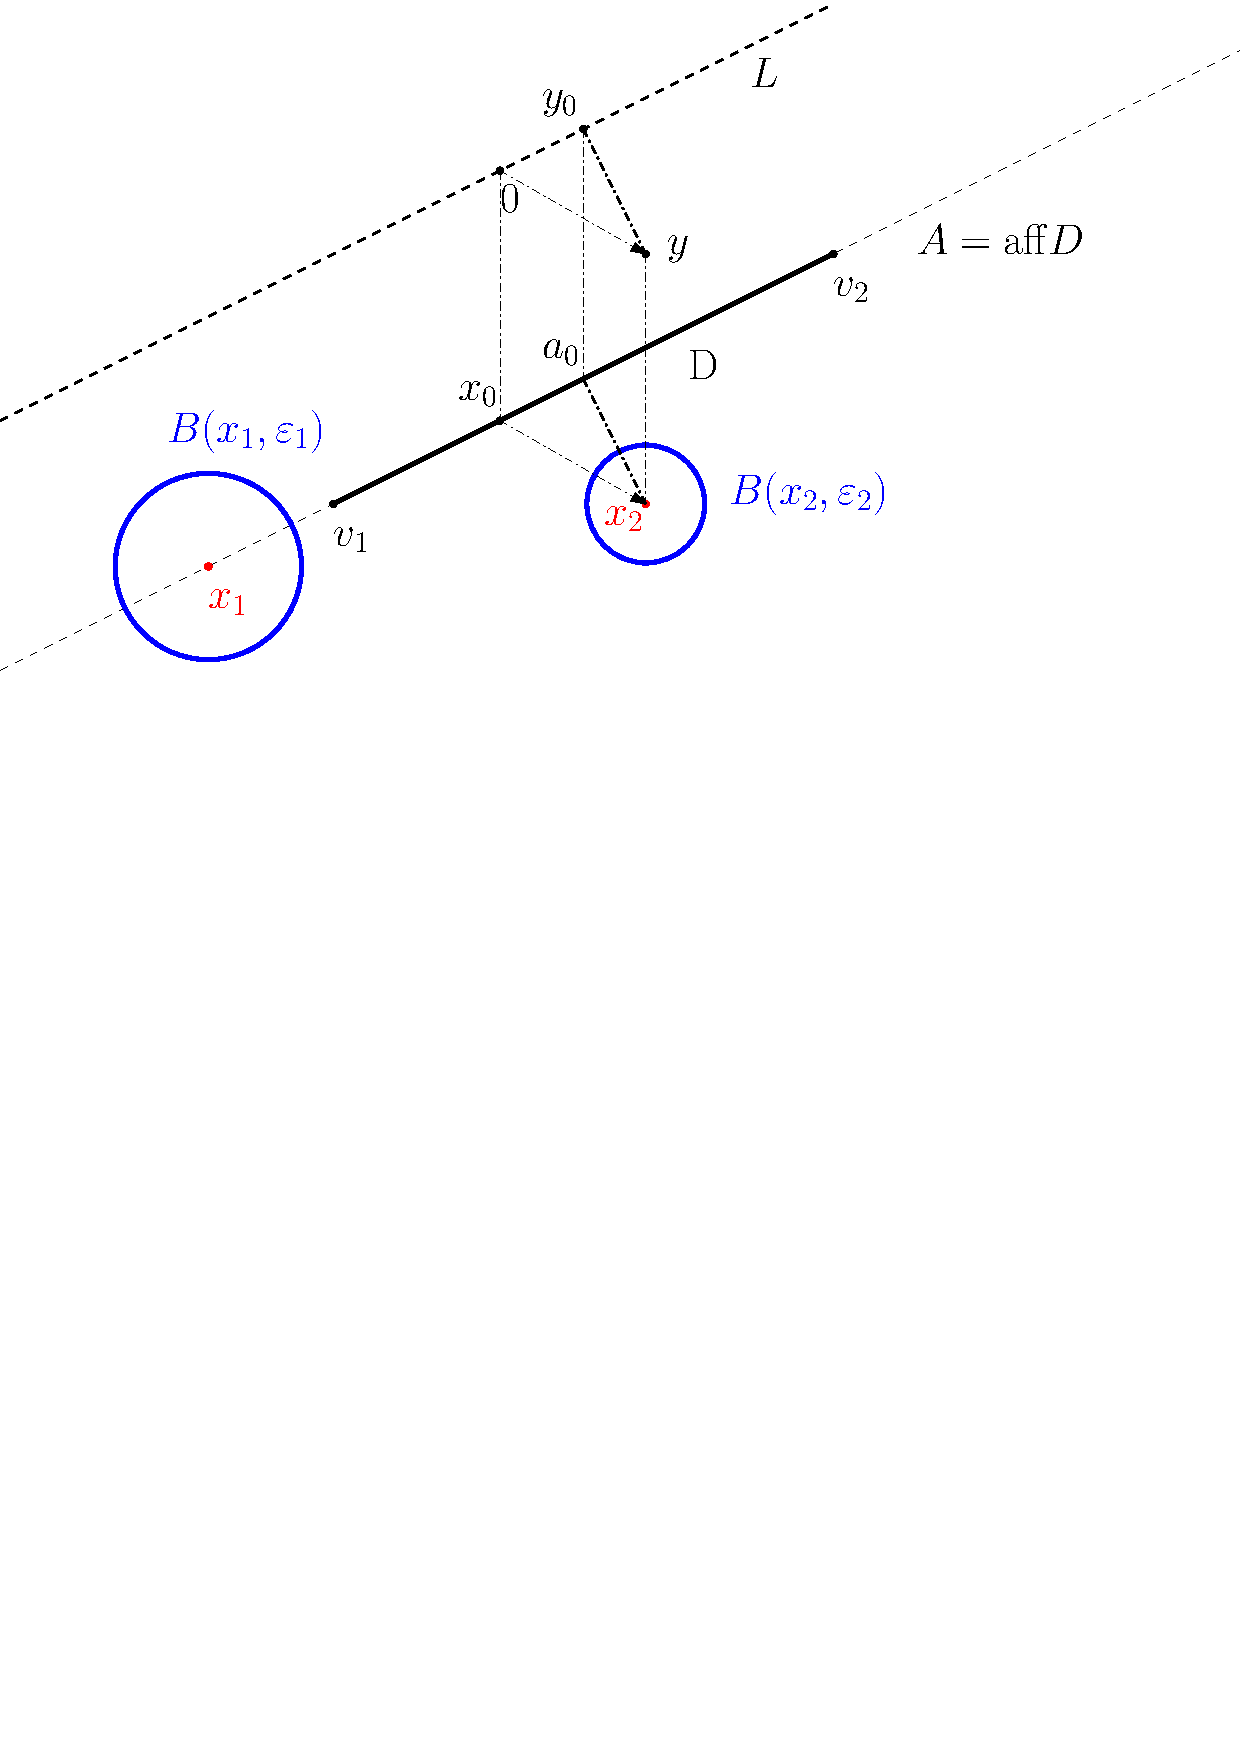
\includegraphics[scale=0.5]{figures/a}
  

  Then, \( D_{1} \) is relatively open. Let \( x \) be a point in \( D_{2} \).

  If \( x \in A \) (denoted as \( x_{1} \) in the figure above),
  then \( x \in A \). Then every neighborhood \( B_{A}(x,
  \varepsilon) \) of \( x \) is in \( D_{1} \), since \( D_{1} \) is open. Now
  consider \( y \in B(x, \varepsilon) \), then either \( y \in A \), implying \(
  y \in B_{A}(x, \varepsilon) \subseteq D_{1} \subseteq D_{2}\) or \( y \in
  A^{c} \subseteq D_{2} \). Hence, in all cases \( y \in D_{2} \), therefore \(
  B(x, \varepsilon) \subseteq D_{2}\).

  If \( x \in A^{c} \) (denoted as \( x_{2} \) in the figure above)
  and assuming \( A = x_{0} + L \) for some linear space \(
  L\). Then, we will prove that there exists \( \varepsilon > 0 \) such that \(
  d(x, a) < \varepsilon\) for all \( a \in A \). Intuitively, the distance from
  \( x \) to \( A \) is one such value for \( \varepsilon \).
  Making thing rigorous,
  let \( u = a - x_{0} \) and \( y = x - x_{0} \), then \( u \in L \). We will
  project \( x \) to \( A \), or equivalently, \( y \) to \( L \). Denote this
  projection as \( y_{0} \). Then, \( y \neq  y_{0} \) and \( d(y, y_{0}) > 0
  \). Pick \( \varepsilon = \frac{1}{2} d(y, y_{0}) \), then \( d(x, a) >
  \varepsilon \) , for every \( a \in A \), which means \( B(x, \varepsilon)
  \cap A = \varnothing \) or \( B(x, \varepsilon) \subseteq A^{c} \subseteq
  D_{2} \).

  In all cases, there exists \( \varepsilon > 0 \) such that \( B(x,
  \varepsilon) \in D_{2} \). Hence, \( D_{2} \) is open and \( D \) is closed.
\end{proof}



\subsection{Hyperplanes and related theorems} % (fold)
\label{sub:Hyperplanes and related theorems}

Consider the feasible for the above problem: \( D = \{x, Ax\ge b\}   \). Then,
one can see that \( D \) is the intersection of sets \( H_{i}=\{x, A^{i}x \ge
b^{i}\}   \) for \( i \) ranging from \( 1 \) to \( m \).

Now, we will have some names for these sets.

\begin{definition}
  A \textbf{hyperplane} is a set \( H \) in the form of \( H = \{x, ax =
  \alpha\}   \). \( H \) splits the whole space into two open sets, which are
  called \textbf{open half-spaces}: \( H_{1} = \{x, ax > b\}   \) and \( H_{2}
  = {x, ax < b} \). There are also \textbf{closed half spaces} \( H_{3} = H_{1}
  \cup H =
  \{x, ax \ge  b\}  \) and \( H_{4} = H_{2} \cup  H = \{x, ax \le  b\}   \). The
  vector \( a^{T} \) is a \textbf{normal} of \( H \).

  Let \( S \subseteq \mathbb{R}^{n} \) and \( x_{0} \in S \). Then, a hyperplane
  \( H = \{x, ax = \alpha\}   \) is a \textbf{supporting hyperplane} of \( S \)
  at \( x_{0} \) iff \( x_{0} \in H \) and either \( S \subseteq H_{1} \) or \(
  S \subseteq H_{2}\), with \( H_{1}, H_{2} \) being the closed half-spaces
  bounded by \( H \).

  Let \( A, B \) be two subsets of \( \mathbb{R}^{n} \). Then, a hyperplane \( H
  \) \textbf{separates} \( A \) and \( B \) if and only if \( H \) splits the \(
  \mathbb{R}^{n}\) space into two closed half-spaces \( H_{1} \) and \( H_{2} \)
  such that \( A \subseteq H_{1} \) and \( B \subseteq H_{2} \).

  If \( H: ax = \alpha \) separates \( A \subseteq H^{+}: ax \ge  \alpha \) and
  \( B \subseteq H^{-}: ax \le \alpha \), then we call this separation
  \textbf{strict} if and only if there exists \( \alpha_{1} \) and \( \alpha_{2}
  \) such that: \( ax_{1} > \alpha_{1} > \alpha > \alpha_{2} > ax_{2} \), \(
  \forall x_{1} \in A, x_{2} \in B \). In other words, this is equivalent to \(
  \inf aA > \sup aB\).
\end{definition}

Before going on proving the important hyperplane theorems, we start with a
simple lemma.

\begin{lemma}
\label{lem:Existence of closest element}
  Let \( S \) be a nonempty, closed set in \( \mathbb{R}^{n} \).
  Then for every \( x_{0} \in S^{c} \), there exists some \( x_{1} \in S \)
  such that \( d(x_{0}, x_{1}) \le d(x_{0}, x), \forall x \in S \).
\end{lemma}

\begin{proof}
  Note that this is basically a minimization problem: \( \min f(x) = d(x_{0}, x), x \in
  S\), then we can use the theorems in the last chapter to prove that a GOS
  exist. We will use Theorem \ref{thr:coercive condition}, which requires \(
  f(x) \) to be (lower semi-)continuous and \( \lim_{x \to \infty} f(x) =
  +\infty \), which are both basic properties of the Euclidean norm.
\end{proof}

\begin{theorem}[Hyperplane Separation Theorem (Closed set-point variant)]
\label{thr:hst-closed-pt}
  Let \( S \) be a nonempty, convex set and denote \( S' \) be its relative
  closure: \( S' = \operatorname{relclo} S = S \cup \operatorname{relbd} S \).
  Then for every \( x_{0} \in S'^{c} \),
  there exists some hyperplane separating \( S' \) (and therefore \( S \))
  and \( \{x_{0}\}   \). Moreover, we can construct a hyperplane that strictly
  separates \( S' \) and \( \{x_{0}\}   \).
\end{theorem}

\begin{proof}
  Let \( x_{1} \) be the closest point on \( \overline{S} \) to \( x_{0} \),
  denote \( d = (x_{1}-x_{0})^{T}\).

  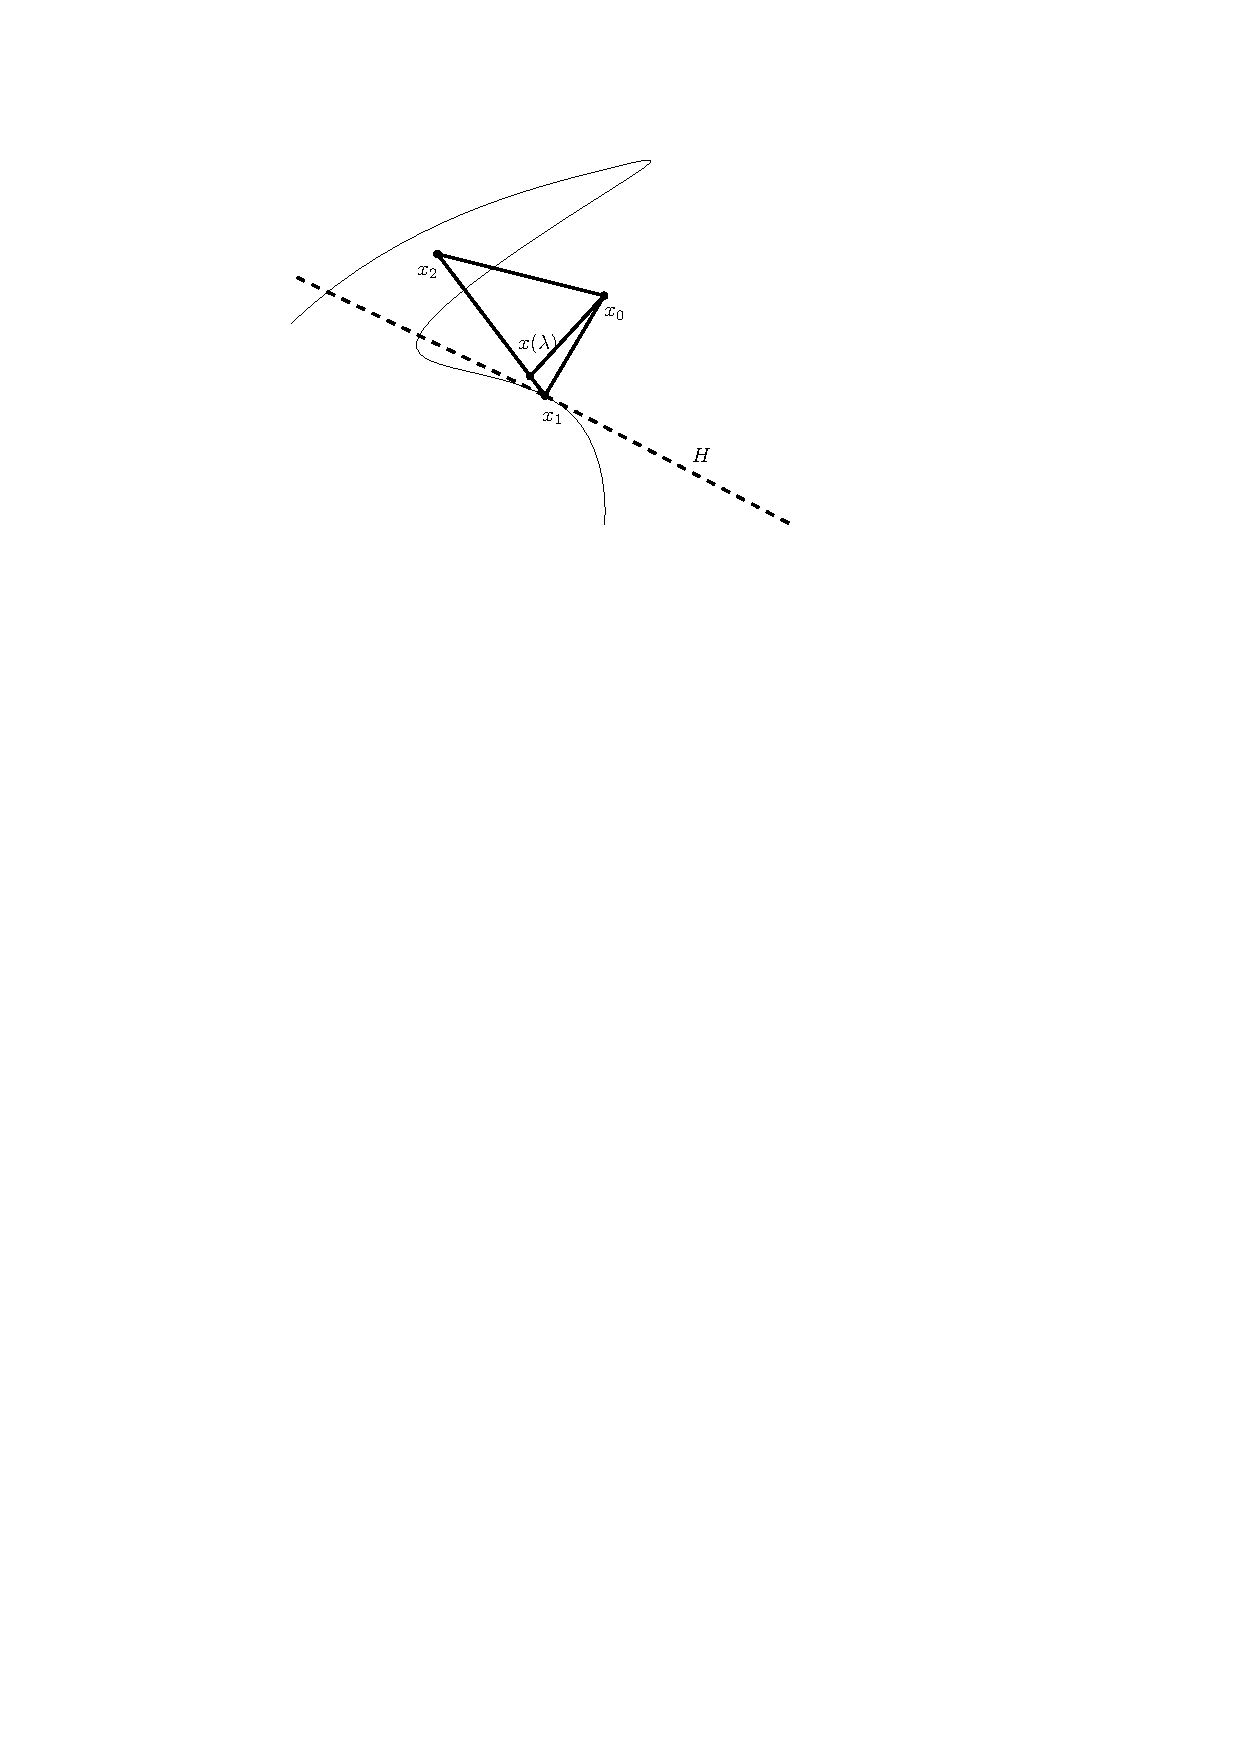
\includegraphics[scale=1.5]{figures/1696779691}

  Then, we will prove that the hyperplane \( H = \{x, dx = dx_{1}\}   \) is a
  supporting hyperplane of \( S \). If this is true, then it's trivial that \( H
  \) separates \( S \) and \( \{x_{0}\}   \).

  Now, we have \( dx_{0}-dx_{1}=-d^{T}d < 0 \), which means that \( x_{1} \in
  H_{1} = \{dx < dx_{1}\}   \). Hence, we need to prove that \( S \subseteq
  H_{2} = \{dx \ge  dx_{1}\}   \), or \( x \in S \implies dx \ge  dx_{1} \).

  Assuming that there is some \( x_{2} \in S \) such that \( dx_{2} < dx_{1} \).
  Consider the lerp between \( x_{2} \) and \( x_{1} \): \( x(\lambda) =
  \operatorname{lerp}(x_{2}, x_{1}, \lambda) \), which must be in \( S \) for
  every \( \lambda \in [0, 1] \)
  \begin{align*}
    x(\lambda) - x_{0} &= \operatorname{lerp}(x_{2}, x_{1}, \lambda) -
    x_{0}\\
                       &= \operatorname{lerp}(x_{2}-x_{1}, 0, \lambda) + (x_{1}
                       - x_{0})\\
                       &= \lambda(x_{2}-x_{1}) + d^{T}\\
  .\end{align*}

  \begin{align*}
    \|x(\lambda)-x_{0}\|^2 &= (\lambda(x_{2}-x_{1}) + d^{T})^{T}(\lambda(x_{2}-x_{1})
    + d^{T})\\
                           &= \|d\|^2 + 2\lambda d(x_{2}-x_{1}) + \lambda
                           ^2\|x_{2}-x_{1}\|^2\\
                           &= \|x_{1}-x_{0}\|^2 + \lambda g(\lambda)
  .\end{align*},
  with \( g(\lambda) = 2d(x_{2}-x_{1}) + \lambda \|x_{2}-x_{1}\|^2 < 0 \) for
  small \( \lambda > 0 \), which means that \( \lambda g(\lambda) < 0 \) and
  therefore \( x(\lambda) \) is closer to \( x_{0} \) than \( x_{1} \), which is
  a contradiction.

  To achieve strict separation, one take \( m = \frac{1}{2}(x_{0} + x_{1}) \),
  the midpoint of the \( [x_{0}, x_{1}] \) segment and construct a hyperplane \(
  H' \) parallel to \( H \), i.e. \( H': dx = \frac{1}{2}d(x_{0} + x_{1}) \),
  then we have \( dx_{0} > dm > dx, \forall  x \in A \), and therefore \( H' \)
  strictly separates \( S' \) and \( \{ x_{0}\}   \).
\end{proof}

\textbf{Remark. } The hyperplane \( H \) constructed above is a supporting
  hyperplane of \( S \) at \( x_{1} \).

\begin{corollary}
\label{cor:Closed convex sets are intersection of closed half-spaces}
  A closed convex set \( S \) is the intersection of the closed half-spaces that
  contains \( S \).
\end{corollary}

\begin{proof}
  If \( x \in S \), then every closed half-space that contains \( S \) contains
  \( x \).

  If \( x \in S^{c} \), then there exists a supporting hyperplane separating \(
  S\) and \( \{x\}   \), which means that \( x \) could not be in the closed
  half-space that \( S \) is in.
\end{proof}


\begin{theorem}[Supporting Hyperplane Theorem]
  \label{thr:Supporting Hyperplane Theorem}
  Let \( S \) be a nonempty convex set and a point \( x_{0} \in \partial S \).
  Then, there exists a supporting hyperplane of \( S \) at \( x_{0} \).
\end{theorem}

\begin{proof}
  In every open ball \( B(x_{0}, \varepsilon_{n}) \), pick a point \( x_{n} \in
  B(x_{0}, \varepsilon_{n}) \cap  S^{c}\). Then, \( \lim_{n \to \infty} x_{n} =
  x_{0}\) if \( \varepsilon_{n} \to  0 \), which we will fix to \( \varepsilon_{n}
  = \frac{1}{n}\) for example.

  Using the previous theorem, there exists hyperplanes \( H_{n} \) separating \(
  S\) from \( \{x_{n}\}   \). Let the normal unit vector of \( H_{n} \) be \(
  d_{n} \), with the convention that \( d_{n}(x-x_{n}) \ge 0, \forall  x \in
  S \).

  Hence, \( d_{n} \) is a sequence on the compact set \( \partial B(0, 1) \),
  which means that there must be a convergent subsequence \( d_{i_{n}} \) that
  converges to \( d \).

  Since \( d_{n}(x-x_{n}) \ge 0 \) for all \( x \in S \), letting \( n = i_{m}
  \) and \( m \to  \infty \), we have \( d(x-x_{0}) \ge 0 \), and therefore \(
  H=\{x, d(x-x_{0})\ge 0\}   \) is a supporting hyperplane of \( S \).
\end{proof}

\textbf{Remark. } This result also holds for all \( x_{0} \in
\operatorname{relbd} S
\), since \( \operatorname{relbd} S \subseteq \partial S \).

\begin{corollary}[Hyperplane Separation Theorem (Set-point variant)]
\label{cor:hst-set-pt}
  Let \( S \) be a nonempty convex set, then for every \( x \in
  (\operatorname{Int} S)^{c} \), there is a supporting hyperplane \( H \) that
  separates \( S \) and \( \{ x\}   \).
\end{corollary}

\begin{proof}
  If \( x \in \partial S \), the supporting hyperplane exists due to Theorem
  \ref{thr:Supporting Hyperplane Theorem}.

  If \( x \in \overline{S}^{c} \), then if \(\overline{S} \) is a convex set,
  there exists a supporting hyperplane of \( \overline{S} \) at \( x \), which
  is also a supporting hyperplane of \( S \) at \( x \), due to Theorem
  \ref{thr:hst-closed-pt}.

  To conclude, one would need to prove that \( \overline{S} \) is convex, using
  the following argument:

    \( \overline{S} \) is the set of all \( x \) such that there exists a
    sequence \( (x_{n})_{n \in \mathbb{N}} \), \( x_{n} \in S, \forall n \in
    \mathbb{N} \) converges to \( x \).

    Consider a point tuple \( A = (A^{1}, A^{2}, \ldots , A^{m}), A^{i} \in
    \overline{S}, \forall i \in 1..m \). To prove \( \overline{S}
    \) is convex, we need to prove that \( x = \mathcal{C}(A, \lambda) \in
    \overline{S} \), for
    all \( \lambda \in \mathbb{R}^{m} \) satisfying the convex conditions.

    Let \( (A_{n})_{n \in \mathbb{N}} \) be the sequence that converges to \( A
    \). Then, \( x_{n} = \mathcal{C}(A_{n}, \lambda) \to  \mathcal{C}(A, \lambda) =
    x\) because of linearity, as \( n \to  \infty \). Note that \( x_{n} \in S
    \) and therefore \( x \in \overline{S} \).
\end{proof}

Finally, we can prove the \textbf{Hyperplane separation theorem}.
\begin{theorem}[Hyperplane Separation Theorem]
\label{thr:Hyperplane Separation Theorem}
  Let \( S_{1}, S_{2} \) be nonempty disjoint convex sets, then there exists a
  hyperplane that separates the sets.

  Furthermore, if either \( S_{1} \) or \( S_{2} \) is compact, then there exists a
  hyperplane that strictly separates \( S_{1} \) and \( S_{2} \).
\end{theorem}

\begin{proof}
  Consider the set \( S = S_{1} - S_{2} = \{s_{1} - s_{2},
  s_{1} \in S_{1}, s_{2} \in S_{2}\}   \).

  \( S \) is convex, since if \( x_{1}-x_{2}, y_{1}-y_{2} \in S_{1}-S_{2} \)
  (s.t. \( x_{1},y_{1} \in S_{1}, x_{2}, y_{2} \in S_{2} \)), then a convex
  combination of the two, which can be written as \(
  \operatorname{lerp}(x_{1}-x_{2},y_{1}-y_{2},\lambda) =
  \operatorname{lerp}(x_{1},y_{1},\lambda) -
  \operatorname{lerp}(x_{2},y_{2},\lambda) \in S_{1}-S_{2} \) due to the fact
  that \( \operatorname{lerp}(x_{i},y_{i}, \lambda) \in S_{i} \).

  Then, using Corollary \ref{cor:hst-set-pt}, there is a hyperplane separating
  \( S_{1}-S_{2} \) and \( \{0\}   \). Moreover, there is one such hyperplane
  that passes through \( 0 \), which could be constructed by slightly modifying
  the proofs of the above theorems. Denote this hyperplane as \( H = \{x, dx \ge
  0\}   \), then we have \( dx_{1} \ge  dx_{2}, \forall x_{1} \in S_{1}, x_{2}
  \in S_{2} \).

  Let \( \alpha = \inf dS_{1}, \beta = \sup dS_{2} \), then we have \( dx_{1}
  \ge  \alpha \ge  \beta \ge dx_{2}, \forall x_{1} \in S_{1},x_{2} \in S_{2} \),
  which yields at least one separating hyperplane of \( S_{1} \) and \( S_{2}
  \): \( H'(\gamma) = \{ dx = \gamma\}   \) for any \( \gamma \in [\alpha,\beta]
  \), which is a nonempty interval.

  When either \( S_{1} \) or \( S_{2} \) are compact, we can prove that \( S \)
  is closed, and \( 0 \notin S = \overline{S} \). Using Theorem
  \ref{thr:hst-closed-pt}, we can construct a hyperplane \( H \) that strictly
  separates \( \{0\}   \) and \( S = S_{1} - S_{2} \).

  \begin{quote}
    Assuming \( S_{1} \) is compact, take \( z \in S^{c} = (S_{1} - S_{2})^{c}
    \). Then, for every \( x \in S_{1} \), \( x - z \in S_{2}^{c} \) (otherwise
    \( z = x - (x - z) \in S \)). Consider \( x' \in B(x, \delta_{1}), z' \in
    B(z, \delta_{2}) \), we have \( x' - z' = (x - z) + (x' - x) - (z' - z) \)
    and therefore \( \|(x' - z') - (x - z)\| \le \|x' - x\| + \|z' - z\| <
    \delta_{1} + \delta_{2} \). Take \( \delta_{1} = \delta_{2} =
    \varepsilon\), we have \( B \left( x, \varepsilon
    \right) - B(z, \varepsilon) \subseteq B(x - z, 2\varepsilon) \).
    Since \( x - z \in S_{2}^{c} \) open, there exists some \( \varepsilon_{x}
    \) such that \( B(x - z, 2\varepsilon_{x}) \subseteq S_{2}^{c} \), and hence
    \( N(x) = B \left( x, \varepsilon_{x} \right)  - B \left( z,
    \varepsilon_{x} \right) \subseteq S_{2}^{c} \).

    Consider this open cover of \( S_{1} \): \( \{B \left( x,
    \varepsilon_{x} \right) , x \in
    S_{1}\}   \), since \( S_{1} \) is compact, there must exist some finite
    subcover \( B \left( x_{1}, \varepsilon_{x_{1}} \right), B(x_{2},
    \varepsilon_{x_{2}}), \ldots ,
    B \left( x_{n}, \varepsilon_{x_{n}} \right) \). Then, \( U = B
    \left( z, \frac{1}{2}\min \{\varepsilon_{x_{1}}, \varepsilon_{x_{2}},
      \ldots, \varepsilon_{x_{n}} .\}
    \right)  \) is an open neighborhood of \( z \) that is totally contained in
    \( (S_{1}-S_{2})^{c} \).

    Assuming \( \exists t \in U \cap (S_{1}-S_{2}) \), then \( B \left( x_{i},
    \varepsilon_{x_{i}} \right) - \{t\} \subseteq S_{2}^{c}  \) and
    \begin{align*}
      S_{2}^{c} &\supseteq \bigcup_{i = 1}^{n} \left( B \left( x_{i},
      \varepsilon_{x_{i}} \right) - \{t\}   \right) \\
                &= \bigcup_{i = 1}^{n} B \left( x_{i}, \varepsilon_{x_{i}}
                \right) - \{t\} \\
                &= S_{1} - \{t\}   
    .\end{align*}
    Write \( t = s_{1} - s_{2} \) for some \( s_{1} \in S_{1}, s_{2} \in S_{2}
    \), we see that \( s_{2} = s_{1} - (s_{1} - s_{2}) = s_{1} - t \in S_{1} -
    \{t\}   \subseteq    S_{2}^{c} \), which is a contradiction.
  \end{quote}
\end{proof}

% subsection Hyperplanes and related theorems (end)

\subsection{Extreme points and faces} % (fold)
\label{sub:Extreme points and faces}

\begin{definition}
  Let \( S \) be a closed convex set. Then a convex \( F \subseteq S \)
  is a \textbf{face} iff \( \forall A \subseteq S \),
  \( \exists x \in F \) is a \textit{strict convex combination} of
  finite \( A \), then \( A \subseteq F \).

  If \( F \neq S \), then \( F \) is called a \textbf{proper face} of \( S \).
\end{definition}

By this definition, any closed, convex set \( S \) is its own face.
Additionally, the empty set \( \varnothing \) is also a face of every closed,
convex set \( S \). These are called as improper faces. The remaining faces,
i.e. faces of \( S \) that is not \( \varnothing \) or \( S \), are
\textbf{proper faces} of \( S \).

\begin{theorem}
\label{thr:No proper faces with full dimensions}
  Let \( S \) be a nonempty closed convex set with \( n = \dim S
  \). Then, if \( F \) is a face with \( n = \dim F \), \( F = S
  \).
\end{theorem}

\begin{proof}
  The idea of the proof goes as follows.
  Assuming \( F \neq  S \), \( F \) is a face of \( S \) and \(
  \dim F = \operatorname{dim} S = n \). Then, take \( x \in S
  \setminus F \) and let \( X \) be a maximum set of affinely independent points
  in \( F \),
  then \( n = \dim F = |X| \).
  If \( X' = X \cup \{x\} \subseteq S   \) is affinely independent, then \( |X'|
  = |X| + 1 = \dim S = n \). This means that \( n = n + 1 \),
  which is a contradiction.

  Hence, \( X' \) could not be affinely independent, which means that \( x \) is
  in the affine hull of \( X \), which will be denoted as \( A \). Note that \(
  F \subseteq \operatorname{aff} X\), hence \( F \subseteq A \).

  Pick a point \( x' \in \operatorname{ri} F \) (we will prove that \(
  \operatorname{ri} F \) is nonempty later), then for small enough \( \lambda
  \), \( x_{0} = \operatorname{lerp}(x', x, \lambda) \) will reside in the open ball \(
  B_{A}(x', \varepsilon) \subseteq F\). Hence, the segment \( [x', x] \)
  intersects \( F \) at \( x_{0} \in F \), which means \( x', x \in F \), which
  contradicts with the face that \( x \in S \setminus F \).

  Finally, we need to prove that \( \operatorname{ri} F \) is nonempty. This
  follows from the following lemma.

  \begin{lemma}
  \label{lem:Nonempty convex set has nonempty interior}
    Every nonempty convex set \( C \) has nonempty interior \( \operatorname{ri}
    C \neq  \varnothing \)
  \end{lemma}

  \begin{proof}[Proof of lemma]
  WLOG, translate \( C \) such that \( 0 \in C \). Then, pick \( n \)
  affinely independent vectors in \( C \) (this is possible since \( n =
  \dim S \)), denoted as \( b_{1}, b_{2}, \ldots , b_{n} \). This
  can be collected into a matrix \( b \), and the representing linear map \(
  f(x) = bx \) will map \( \mathcal{S} = \operatorname{conv} \{0, \mathbf{e_{1}},
  \mathbf{e_{2}}, \ldots, \mathbf{e_{n}} \}   \) to \( \operatorname{conv} \{0,
  b_{1}, b_{2}, \ldots , b_{n}\} \subseteq C   \). This map preserves (relatively)
  interior points, and the set \( \mathcal{S} \) trivially have a nonempty interior,
  therefore \( C \) must have at least an interior point.
  \end{proof}
\end{proof}

Aside from the nonproper faces, there is also a class of faces that is very
special.

\begin{definition}
  Let \( S \) be a subset of \( \mathbb{R}^{n} \).

  If \( S \) is convex, then \( x \in S \) is an \textbf{extreme point} if and only if
  it could not be written as a strictly convex combination of a collection
  of points in
  \( S \) not containing \( x \). In other words, \( x \in S \) is an extreme
  point if for every \( y, z \in S \setminus \{x\}, w \in (0, 1)   \), we have
  \( x \neq \operatorname{lerp}(y,z,w) \).

  Equivalently \( x \) is an extreme point of \( S \) if and only if \( \{x\}
  \) is a face of \( S \).
\end{definition}

For closed sets, we can prove that all of its faces are closed.

\begin{theorem}
  If \( F \) is a face of a closed, convex set \( S \), then \( F \) is also
  closed.
\end{theorem}

\begin{proof}
  For nonproper faces \( F \), the theorem is trivial. We will only consider
  proper faces \( F \).

  \centerline{
    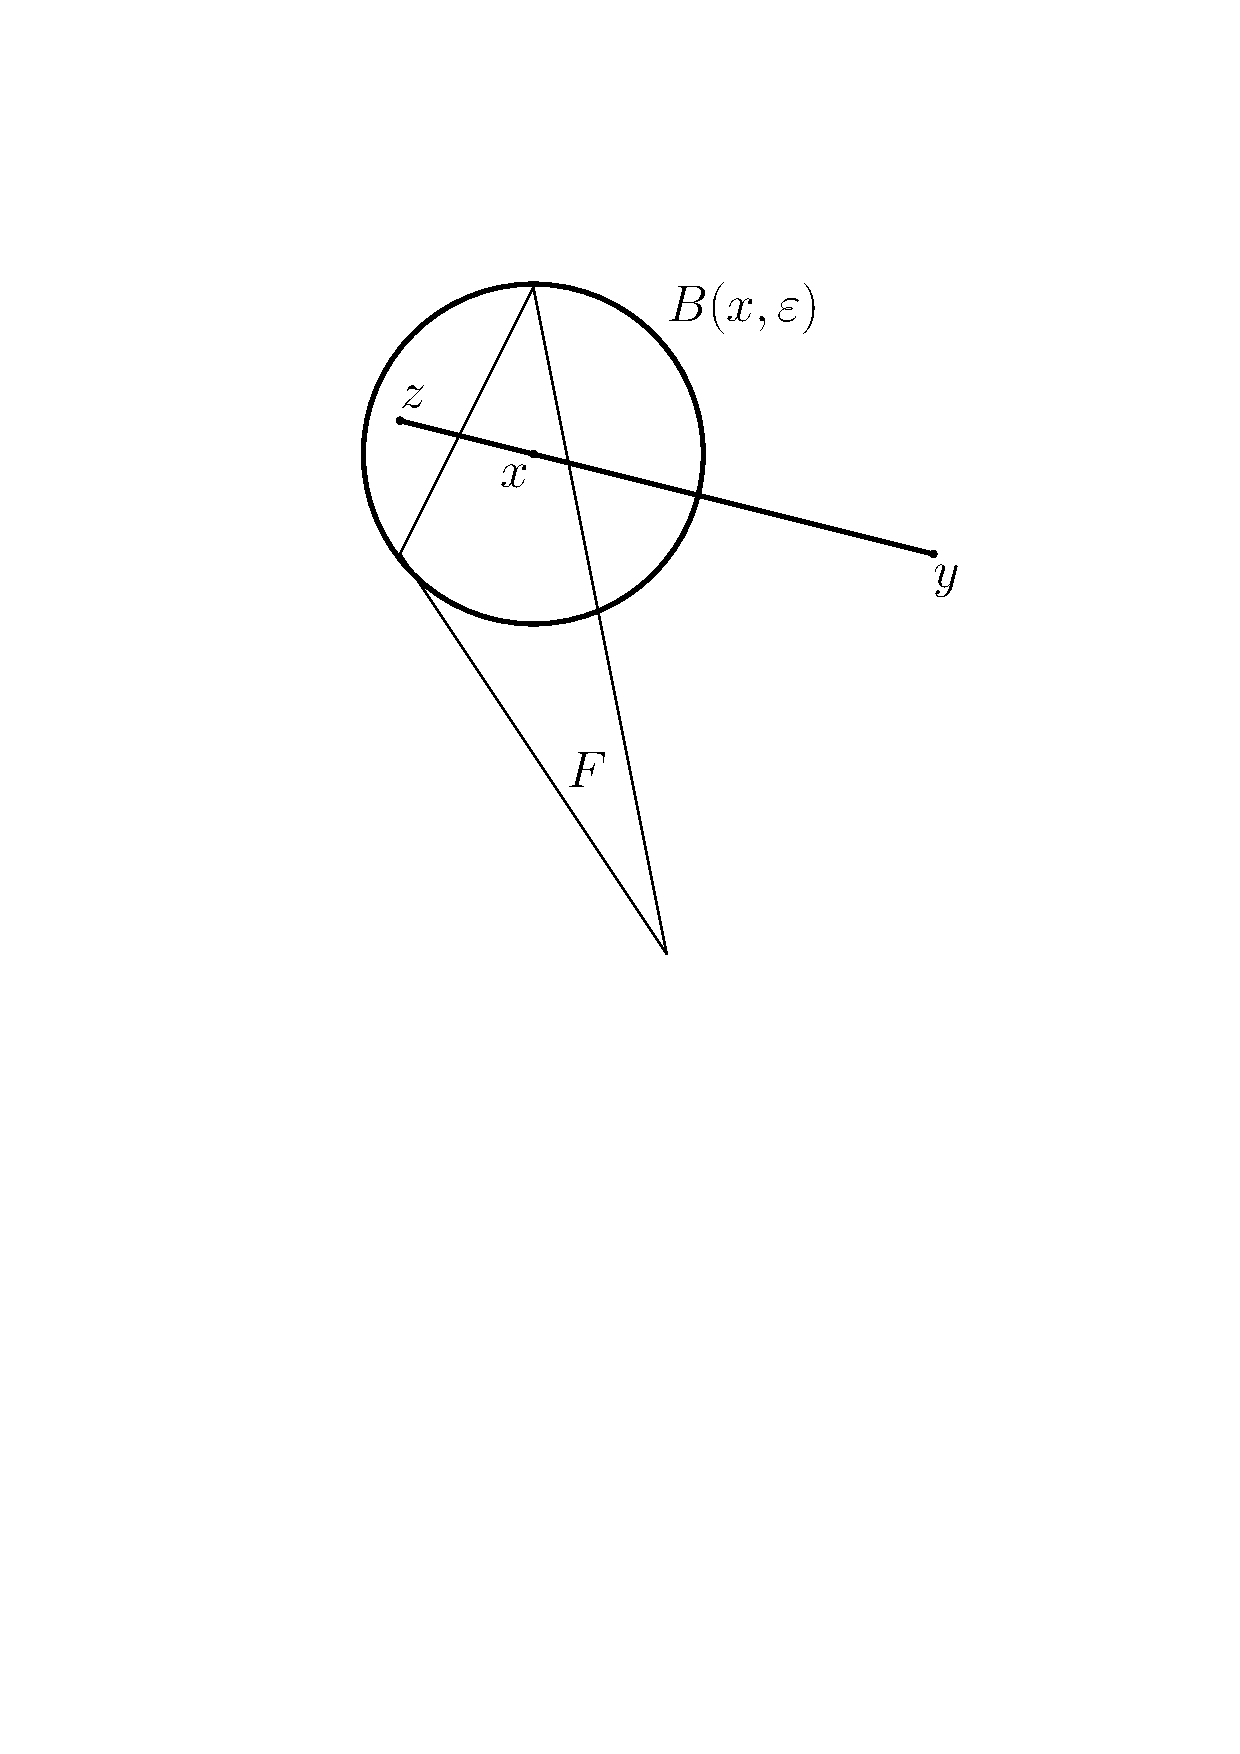
\includegraphics[scale=0.5]{figures/1696828548}
  }

  Since relatively closed and closed are the same thing, the relative closure of
  a set is simply its closure. Hence, there is no need to differentiate between
  the relative closure of \( F \) and \( \overline{F} \). Another important
  thing to note is that \( \overline{F} \subseteq S \), because of the
  minimality of closures.

  Using Lemma \ref{lem:Nonempty convex set has nonempty interior}, we have proven
  that every nonempty convex set has a nonempty interior. Pick \( x \in
  \operatorname{ri} F \), then for all \( y \in \overline{F}
  \setminus \{ x\}   \), and consider the ray \( R = \{x + \lambda (x - y),
  \lambda \ge  0\}   \).

  Consider the intersection \( I \) of the ray with \( \overline{F} \). Since \(
  \overline{F}\) and \( R \) are closed, \( I \) must be closed and convex, \( I
  \) is also a closed and convex set.

  Consider the set \( L = \{ \lambda \ge 0, x + \lambda(x - y) \in
  \overline{F}\}   \). This set is nonempty (\( 0 \in L \)), and therefore has
  a supremum \( \lambda_{0} = \sup L \ge 0 \). Then, there exists a
  diffeomorphism between \( L \) and \( I \): \( f(\lambda) = x + \lambda(x - y)
  \), and therefore \( L \) is convex and closed. Hence, it is trivial to prove
  that \( L \) contains the segment \( [0, \lambda_{0}] \) and because of the
  maximality of \( \lambda_{0} \), \( L = [0, \lambda_{0}] \).

  We have two cases.
  \begin{itemize}
  \item If \( \lambda_{0} = 0 \), then \( L = \{0\}   \). Then every point \(
    z_{\lambda}
    = x + \lambda(x - y) \notin \overline{F}\). For every neighborhood \( B(x,
    \varepsilon) \)
    of \( x_{0} \) with relative to \( A = \operatorname{aff} F \), there exists
    \( z_{\varepsilon} \in B(x, \varepsilon) \) not in \( \overline{F} \) and \(
    z_{-\varepsilon} \in [x, y] \subseteq \overline{F} \), for arbitrarily small
    \( \varepsilon > 0 \). Then, \( x \in \operatorname{relbd} F \), which is a
    contradiction with \( x \in \operatorname{ri} F \).
  \item If \( s > 0 \), then \( x \) is a strictly convex combination of \( y \)
    and \( z = x + s(x - y) \). Then, \( y, z \in F \) due to the definition of
    faces.
  \end{itemize}

  Hence, \( y \in F \) for every \( y \in \overline{F} \), which means \(
  \overline{F} \subseteq F \), or \( F = \overline{F} \) is a closed set.

  \iffalse
  \begin{itemize}
    \item Let \( A \subseteq S \) be a finite set such that \( x =
      \mathcal{C}(A, \lambda) \in S \), then \( A \subseteq F \) because of the
      definition of faces. Using the definition once more for \( F' \), we have
      \( A \subseteq F' \), which means \( F' \) is a face of \( S \).


    \item 
    \item Pick \( x \in F \) (if \( F = \varnothing \) then \( F \) is easily
      closed). Let \( L \) be the linear space that is parallel to \(
      \operatorname{relclo} F = F \cup \operatorname{relbd} F \), the relative
      closure of \( F \), since \( x, y \in F \) we have \( y - x \in L \).
      Then, one can pick \( z = x + \lambda(x - y) \) for some \( \lambda \ge 0
      \) such that \( z \in B(x, \varepsilon) \subseteq \operatorname{^{i} } F
      \), which means \( x \) is now a strict convex combination of \( y \) and
      \( z \). Since \( F \) is a face, \( y, z \in F \). Hence, \(
      \operatorname{relclo} F = F \), which means that \( F \) is closed.

      To make the proof more rigorous, we need to prove \( \operatorname{relclo}
      F \subseteq S\), which comes from \( S \) being a closed convex set. This
      is a rather trivial result, coming from the fact that the closure of a set
      \( F \) is the minimal closed set containing \( F \).
  \end{itemize}
  \fi
\end{proof}

\textbf{Remark.} The condition \( F \) convex in the definition of a face is very
important, without it the above theorem fails to hold.

For example, take \( S = \{(x, y), x^2 + y^2 \le  1\}   \), the closed unit
circle. This set is convex, closed and bounded. The upper-half circle, denoted
as \( U = \{(x, y) \in S, x^2 + y^2 = 1, y > 0\}     \) is a "face" of \( S \)
(if convexity is not needed for faces), but it is not closed. This is due to \(
\operatorname{ri} F = \varnothing\), breaking down the whole proof above.

Consider a face \( F' \) of a face \( F \) of \( S \). If \( x \in F' \), then
every strictly convex combination \( x = \mathcal{C}(A, \lambda), A \subseteq
F\), implies that \( A \subseteq F' \). Moreover, since \( x \in F \), the
condition \( x = \mathcal{C}(A, \lambda), A \subseteq S \) implies \( A
\subseteq F \). Hence, for every strictly convex combination \( x =
\mathcal{C}(A, \lambda), A \subseteq S \), we can deduce that \( A \subseteq F'
\). In other words, \textbf{faces of faces are also faces of the set}.

Since extreme points form a special class of faces, we also have a corollary of
this fact: \textbf{extreme points of faces are also extreme points of the set}.

Hence, we have the following theorem.

\begin{theorem}[Faces and extreme points of faces]
\label{thr:Faces and extreme points of faces}
  Let \( F \) be a face of a convex set \( S \). Then:
  \begin{itemize}
  \item Every face \( F' \) of \( F \) is a face of \( S \).
  \item Every extreme point \( x_{0} \) of \( F \) is an extreme point of \( S
    \).
  \end{itemize}
\end{theorem}

Now, we will look at a class of faces that will be very important for our
purposes.

\begin{theorem}[Exposed faces]
\label{thr:Exposed faces}
  Let \( C \) be a convex set that lies on one closed half-space of the
  hyperplane \( H: ax = \alpha \). Then, the intersection of \( C \) and \( H
  \), \( F = C \cap H = \{x \in C, ax = \alpha\}   \), called an \textbf{exposed
  face induced by} \( H \), is a face.
\end{theorem}

\begin{proof}
  Assuming \( C \subseteq H' = \{x \in \mathbb{R}^{n}, ax \le  \alpha\}   \).
  Then assuming \( \exists y, z \in C \) such that \( \operatorname{lerp}(y, z,
  \lambda) \in F \) for some \( \lambda \in (0, 1) \) and \( y \neq  z \).

  Now,
  \begin{align*}
    \operatorname{lerp}(y, z, \lambda) \in F &\iff a\operatorname{lerp}(y, z,
    \lambda)\\
                                             &\iff \operatorname{lerp}(ay, az,
                                             \lambda) = \alpha
  .\end{align*}
  
  Since \( y, z \in C \), \( ay, az \le \alpha \). Then, \(
  \operatorname{lerp}(ay, az, \lambda) \le \alpha \) for some \( \lambda \in (0,
  1) \). Equality occurs if and only if \( ay = az = \alpha \), which means \(
  y, z \in F \). Hence, \( F \) is a face.
\end{proof}

This theorem gives us a way to find a whole class of faces of an arbitrary
(most optimally compact) convex set in an intuitive sense. Simply move a
hyperplane along its normal until it hit the set, and then the intersection
would be a face of the convex set.

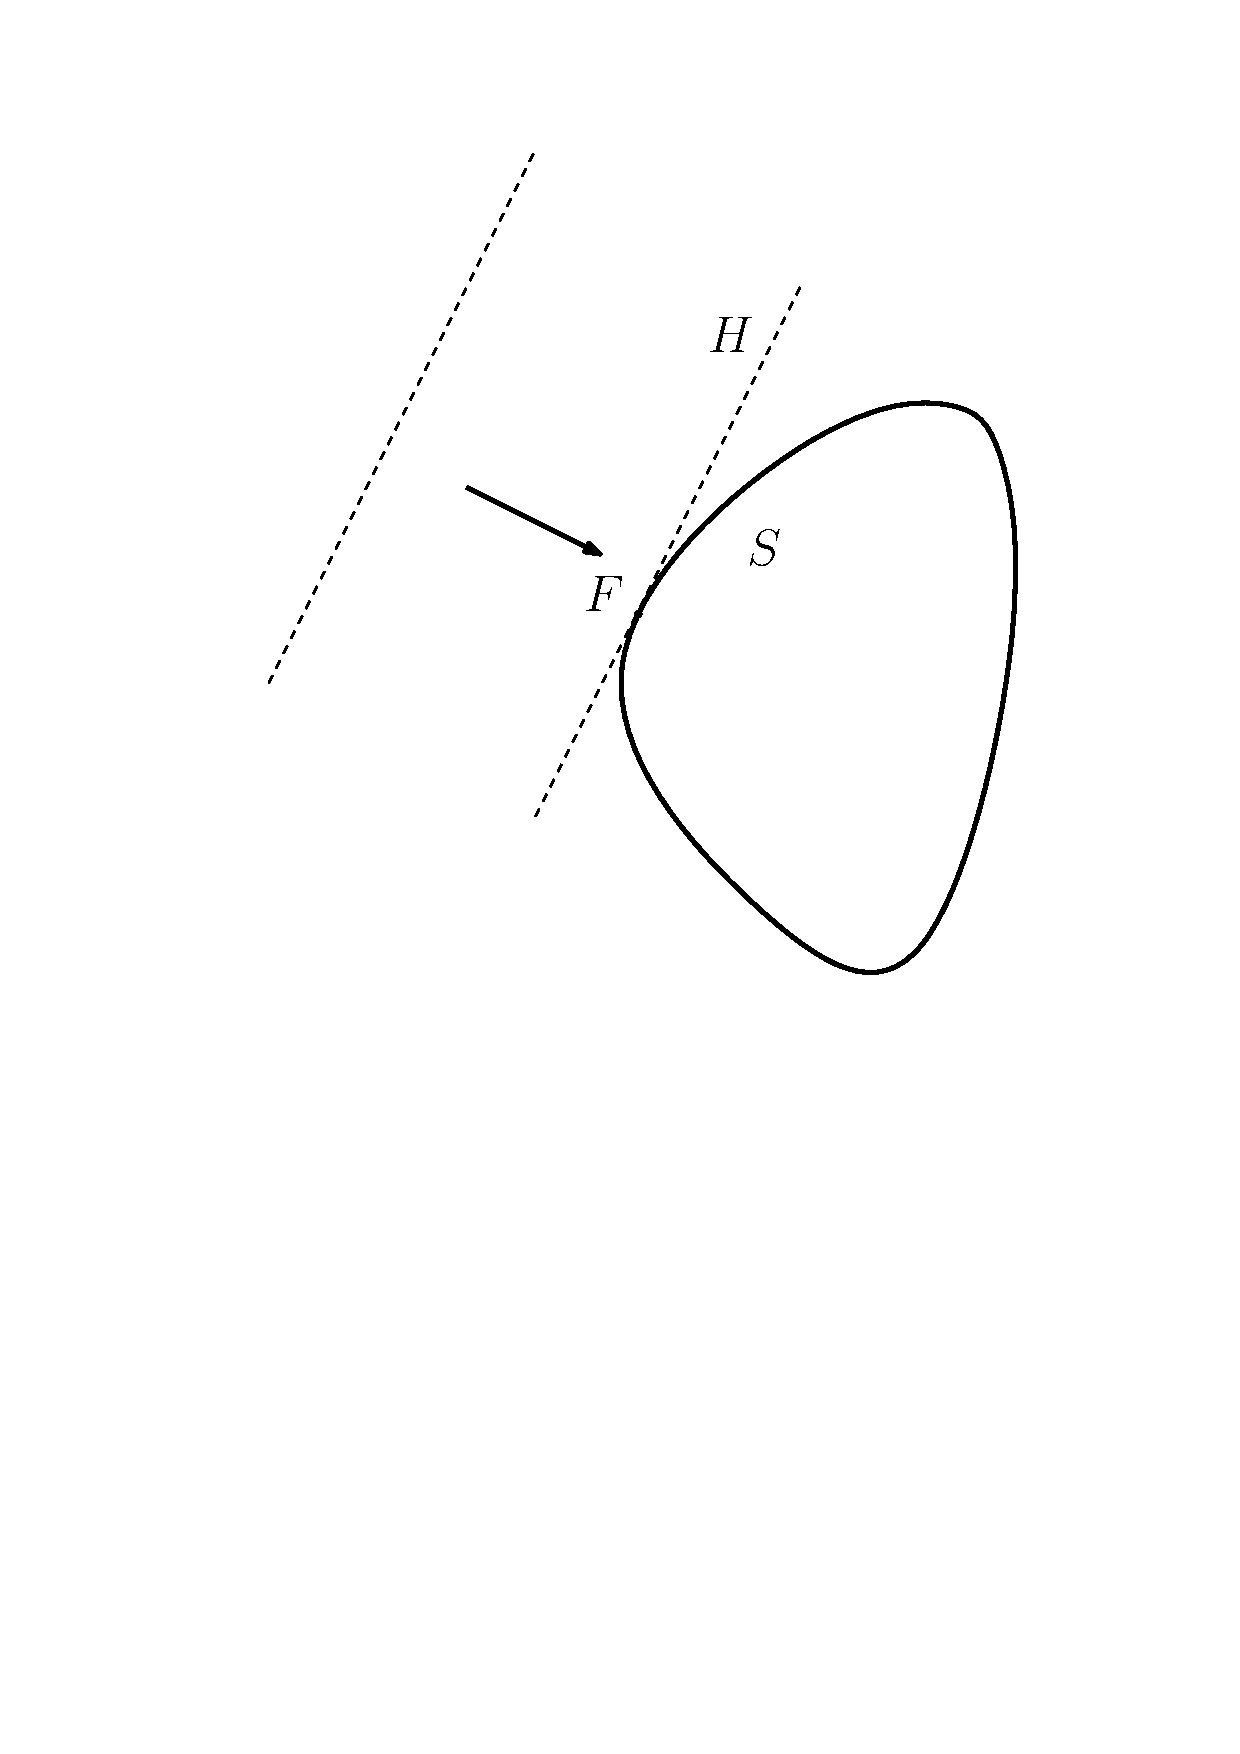
\includegraphics[scale=0.5]{figures/1696891724}

Now, if we let \( H \) be a supporting hyperplane of \( S \) at some point
\( x_{0} \in \operatorname{relbd} S \). Then, \( F = S \cap H \) is an exposed
face, and furthermore, by Lemma \ref{lem:Supporting Hyperplane Theorem (Stronger
variant)}, there exists \( y \in S \) such that \( y \notin H \). Then, \( F
\neq  S \) and therefore \( F \) is a proper face of \( S \).

The other direction, \( x_{0} \in F \) is a proper face of \( S \) implies \(
x_{0} \in \operatorname{relbd} S \), also holds. Let \( A = \operatorname{aff} S
\), then assuming there exists \( x_{0} \in \operatorname{ri } S \cap F \). This
implies that \( B_{A}(x_{0}, \varepsilon) \in S \) for some \( \varepsilon > 0
\), and in this ball we can pick two points \( y \) and \( z \) such that \( x =
\frac{1}{2}(y + z) \). In fact, for every \( y \in B_{A}(x_{0}, \varepsilon) \),
there exists \( z = 2x_{0} - y \) satisfying this property and since \( F \) is a
face, \( y, z \in F \). Hence, \( B_{A}(x_{0}, \varepsilon) \subseteq F \).
Note that \( \dim B_{A}(x_{0}, \varepsilon) = n \), and by Theorem
\ref{thr:No proper faces with full dimensions}, we have a contradiction.

Hence, we have the following lemma.

\begin{lemma}
\label{lem:Points on relative boundary lies on a proper face}
  Let \( S \) be a closed, convex set. Then \( x_{0} \in \operatorname{relbd}
 S \) iff \( x_{0} \) lies on a proper face of \( S \).
\end{lemma}

\iffalse
This relationship between faces and supporting hyperplane gave us a thought:
\textit{For some point \( x \) on some face \( F \), will the supporting
hyperplane at \( x \) contain all of \( F \)}? The answer is in general, no, for
example here:
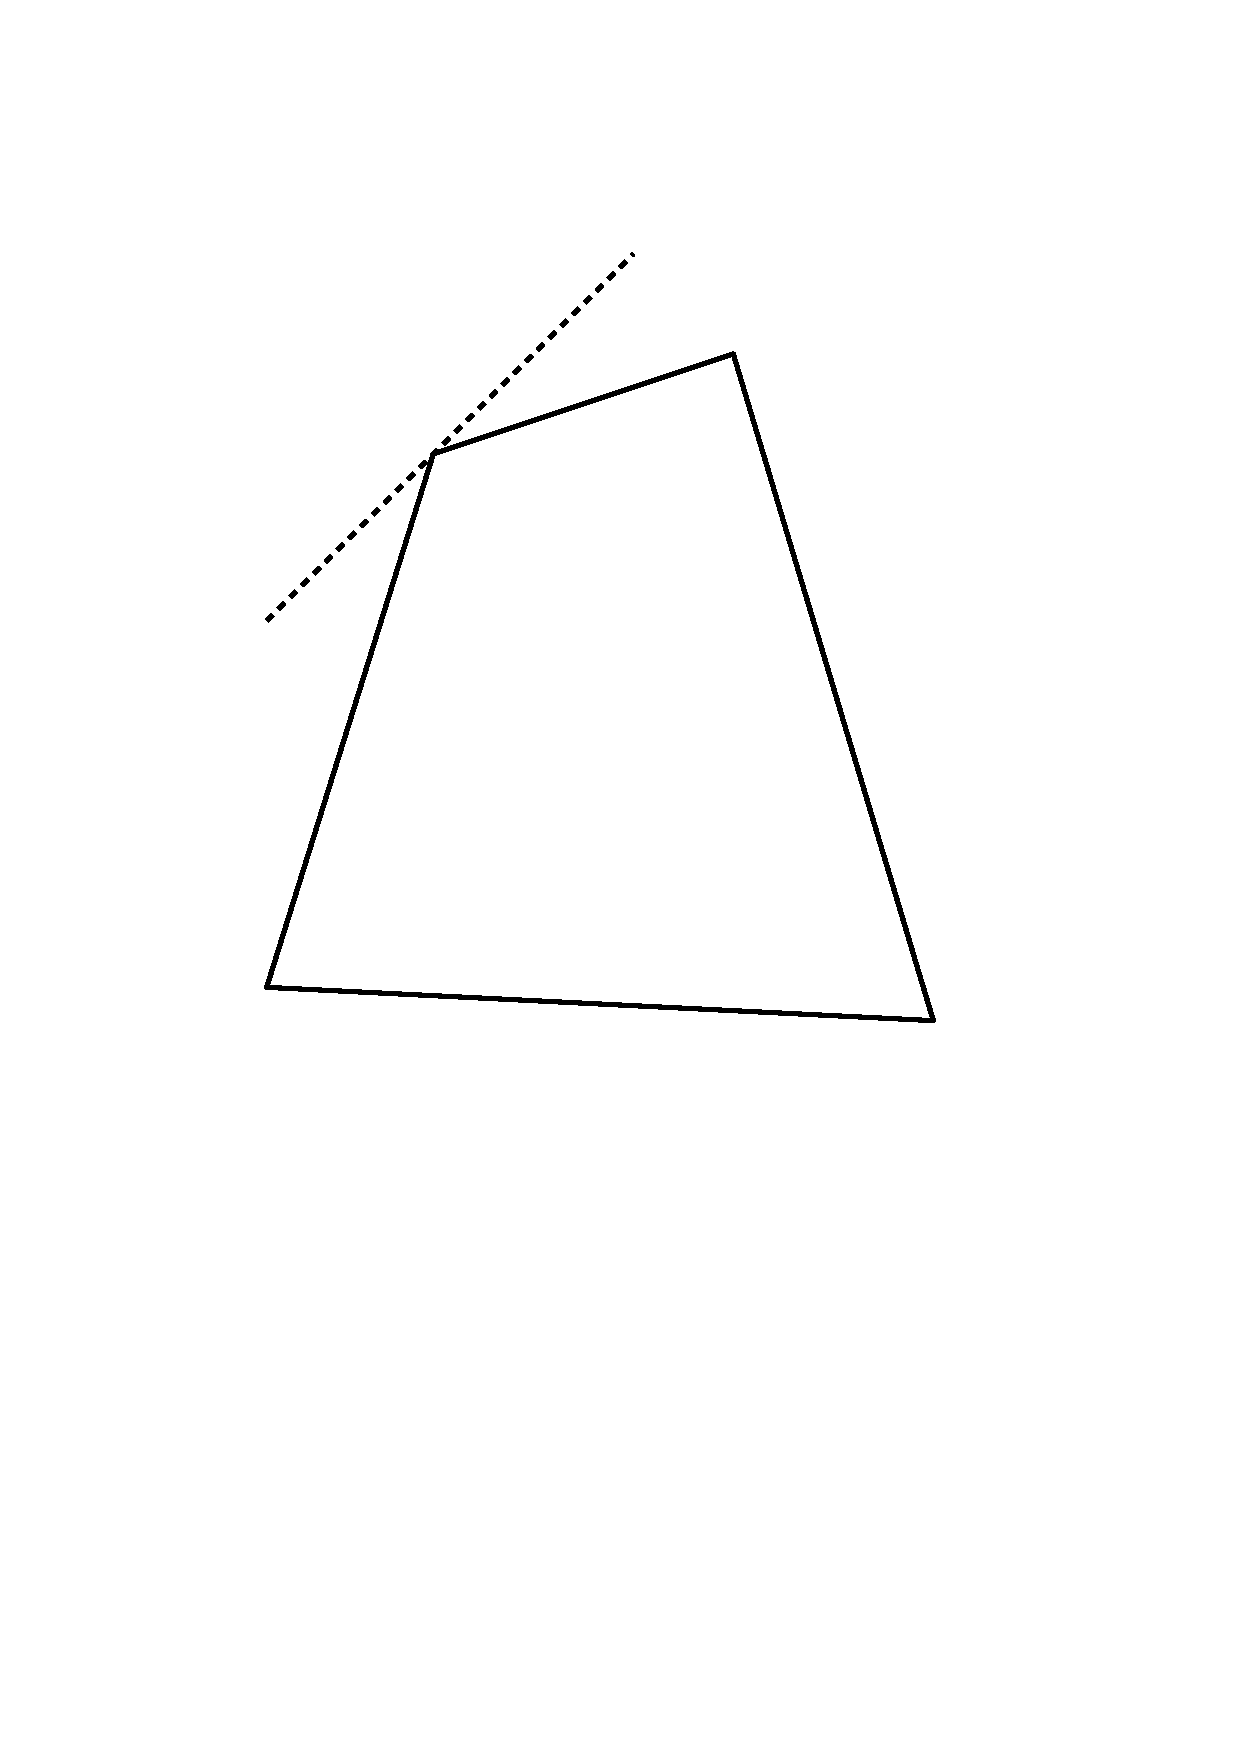
\includegraphics[scale=0.5]{figures/1697082969}

However, if one let \( x \in \operatorname{ri} F \), the result is actually
true, according to the following theorem.
\fi

Now, we will consider some lemmas that will greatly help us in proving the
\textbf{Krein-Milman theorem}.

  \begin{lemma}[Supporting Hyperplane Theorem (Stronger variant)]
  \label{lem:Supporting Hyperplane Theorem (Stronger variant)}

  Let \( C \subseteq \mathbb{R}^{n} \) and \( x_{0} \in \operatorname{relbd} C \).
  Then, there exists hyperplane \( H = \{x, ax = \alpha\}   \) that supports \(
  C\) at \( x_{0} \) such that \( \exists y \in C, ay \neq  \alpha \).
  \end{lemma}

  Theorem \ref{thr:Supporting Hyperplane Theorem} showed that without the last
  condition, \( H \) always exist. This last condition is the only difference
  between the hyperplanes from the basic theorem and this stronger variant.

  Note that this theorem is no longer true for every \( x_{0} \in \partial C \),
  for example considering the segment \( [v_{1}, v_{2}] \) in \( \mathbb{R}^2
  \), its boundary is the whole segment, but one could not construct such a
  supporting hyperplane from a point \( v \) relatively inside the segment, for
  example \( v = \frac{1}{2}(v_{1} + v_{2}) \).

  \begin{proof}[Proof of lemma]
    Let \( A = \operatorname{aff} C, n = \dim_A \). \( n = 0 \) is
    the trivial case, which we will not get into. Consider \( n \ge  1 \).
    
    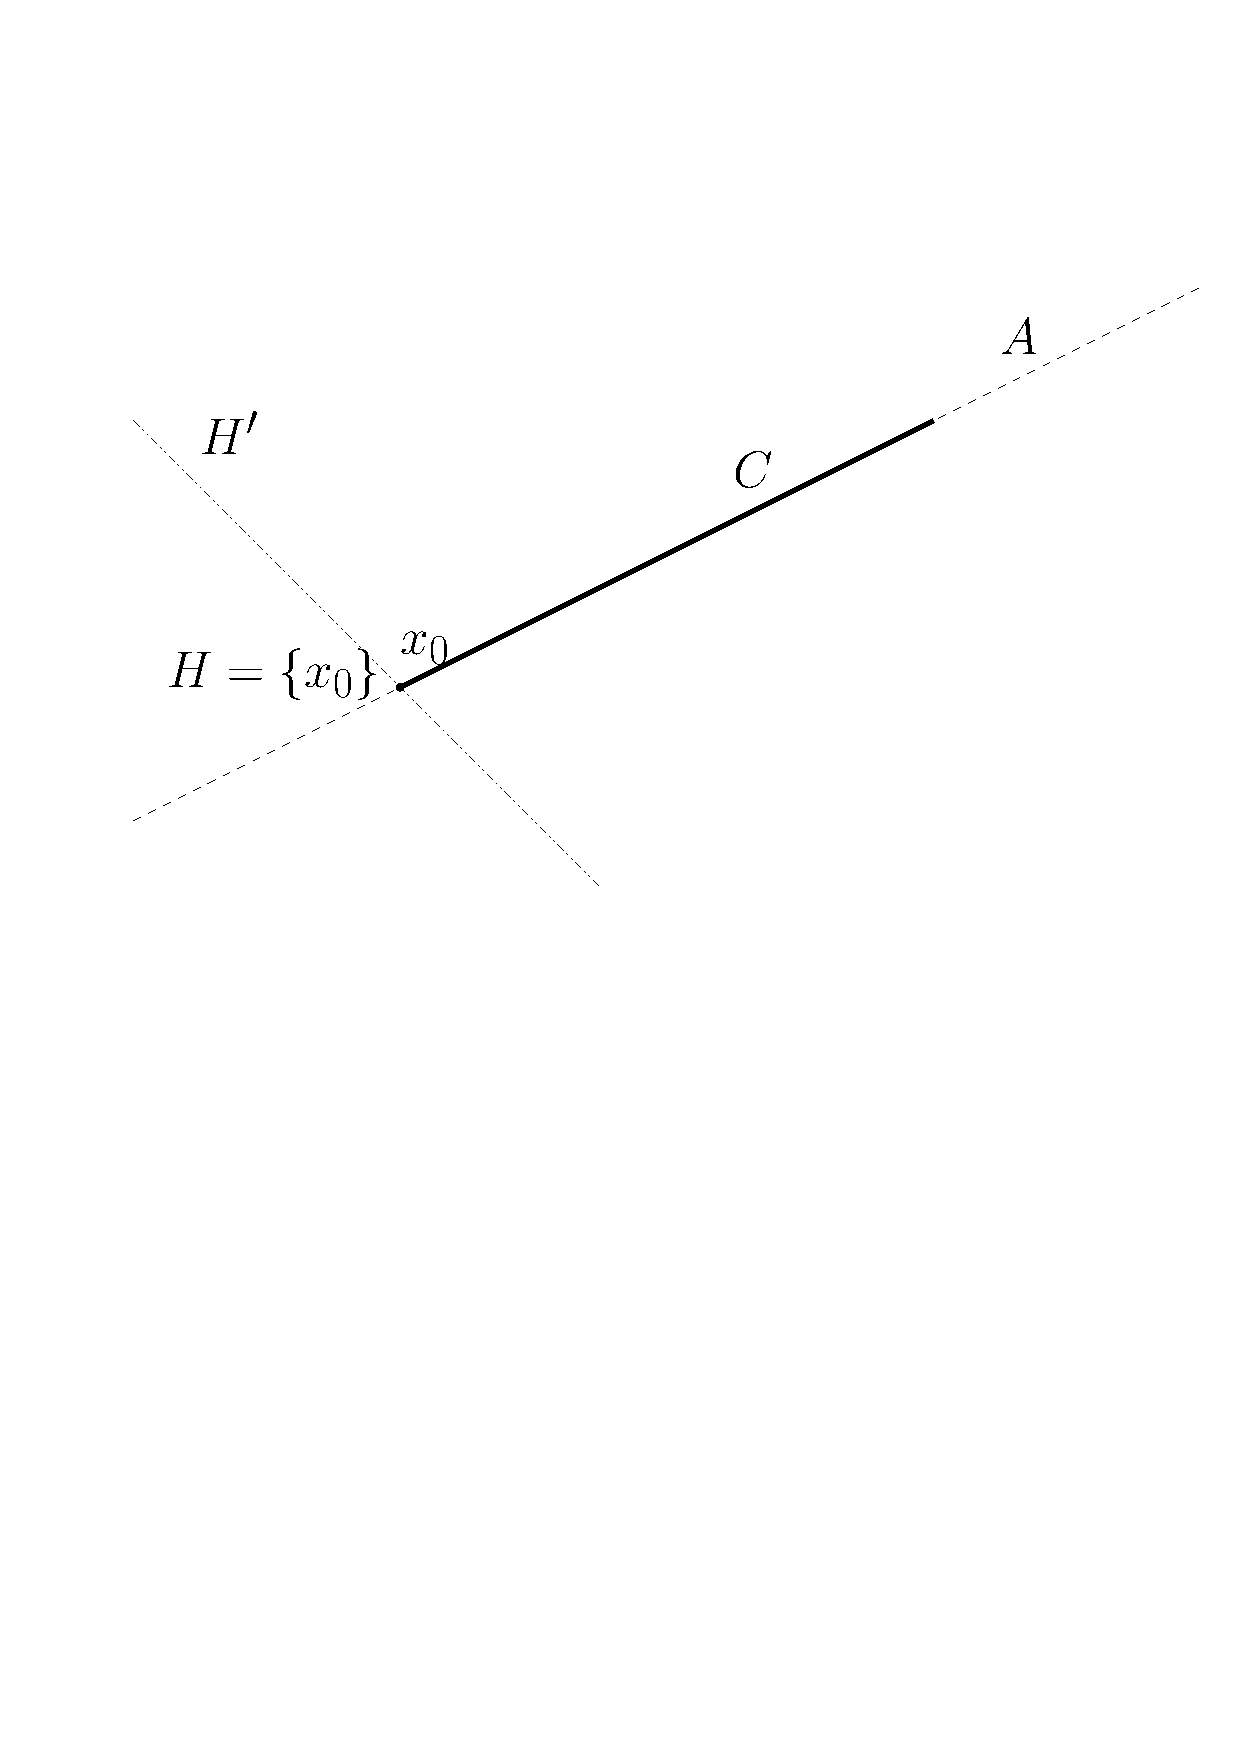
\includegraphics[scale=0.5]{figures/1696827875}

    Then, in the topological space \( (A, \Sigma') \) generated by \( (A, d) \),
    using Theorem \ref{thr:Supporting Hyperplane Theorem}, there exists a
    \( A \)-hyperplane \( H \subseteq A \) that supports \( C \). Then, assuming
    that \( \forall y \in C, y \in H \), which means \( C \subseteq H \). Since
    \( H \) is an affine set and the fact that \( A \) is the minimal affine set
    that contains \( C \), we must have \( A \subseteq H \). Note that \( H
    \subseteq A \), therefore \( A = H \), which means that \(
    \dim A = \operatorname{dim} H \), which could not happen.

    Hence, \( \exists y \in C, y \in H \). Construct a \( \mathbb{R}^{n}
    \)-hyperplane that contains \( H \) and only intersect \( A \) at \( H \),
    we can see that \( H' \) is the hyperplane that satisfies all of the
    conditions we need.
  \end{proof}

\begin{theorem}[Krein-Milman Theorem]
\label{thr:Krein-Milman Theorem}
  A compact and convex set \( S \) is the convex hull of the set of its extreme
  points.
\end{theorem}

\begin{proof}
  We will use induction on \( n = \dim S \). This is easy to
  verify for \( n = -\infty \) (\( S = \varnothing \)) and \( n = 0 \) (\( S =
  \{x_{0}\}   \)).

  For \( x \in S \), we have two cases:

  \begin{itemize}
  \item If \( x \in \operatorname{relbd} S \), then \( x \) lies on some proper
    face \( F \) of \( S \) with \( \dim F < \operatorname{dim} S
    = n\). Since \( F \) is also compact due to Theorem \ref{thr:Faces and
    extreme points of faces}, \( x \) is a convex combination of the
    extreme points of \( F \), which are also extreme points of \( S \).

  \item If \( x \in \operatorname{ri} S \), consider a line \( L \) passing
    through \( x \) that is contained in \( \operatorname{aff} S \). This line
    intersect \( S \) at some set \( S' \), which is a nonempty (\( x \in S'
    \)), convex (since \( S \) is convex), one-dimensional (since a line is
    one-dimensional). Intuitively (or rigorously using infimums and supremums),
    we can deduce that \( S' \) is a line segment, with the endpoints of \( S'
    \), \( y \) and \( z \) must reside on \( \operatorname{relbd} S \). Then,
    \( y \) and \( z \) are convex combinations of extreme points of \( S \),
    and since \( x \in [y, z] \), \( x \) is a convex combination of \( y \) and
    \( z \), we can see that \( x \), in fact, is a convex combination of the
    extreme points of \( S \).
  \end{itemize}
\end{proof}

% subsection Extreme points and faces (end)

\subsection{Recession directions and lineality space} % (fold)
\label{sub:Recession directions and lineality space}

\begin{definition}
  Let \( S \) be a subset of \( \mathbb{R}^{n} \).

  If a vector \( v \) satisfies, \( x + tv \in S \) for every \( x \in S \), \(
  t \ge  0\), then \( v \) is a \textbf{recession direction} of \( S \).

  A recession direction \( v \) is called a \textbf{extreme direction} if it is
  not a strictly convex combination of any collection of recession directions
  not containing directions in the form \( kv \) for scalars \( k \in \mathbb{R}
  \).

  The set of all recession directions of \( S \) is called a \textbf{recession
  cone} of \( S \), denoted as \( \operatorname{rec} S \).
\end{definition}

Here is an equivalent definition for recession directions, stated as a theorem.

\begin{theorem}
\label{thr:Recession direction only needs one point}
  Consider a closed and convex set \( S \) and \( x_{0} \in S \).
  If \( x_{0} + t d \in S \) for
  every \( t \ge  0 \) and some vector \( d \), then \( d \) is a recession
  direction of \( S \).
\end{theorem}

\begin{proof}
  Assuming \( d \) is not a recession direction of \( S \), then there exists \(
  x_{1} \in S, t_{0} \ge 0\) such that \( x_{1}+t_{0}d \notin S = \partial S \).

  Hence, by Theorem \ref{thr:Supporting Hyperplane Theorem}, there exists \( a
  \in \mathbb{R}^{n}, \alpha \in \mathbb{R} \) such that \( a(x_{1}+t_{0}d) >
  \alpha\ge ax, \forall  x\in S \).

  Then, one can see that \( a(x_{1}+t_{0}d) > a(x_{0}+t_{1}d) \) for every \(
  t_{1} > 0 \), or equivalently \( a(x_{1}-x_{0}) > (t_{1}-t_{0})ad \) for every
  \( t_{1} > 0 \). Since the LHS is finite and \( t_{1}  \) can approach \(
  +\infty \), we must have \( ad \le  0 \), which means \( a(x_{1}+t_{0}d) <
  ax_{1} \le \alpha \), which is a contradiction with the fact that \( x_{1}
  \in S \).
\end{proof}

Do note that this theorem is only true for closed and convex sets, so convex
alone is not enough. There is a simple counterexample: \( S = \{(x, y) \in
\mathbb{R}^2, y > 0\} \cup \{(x, 0), x \in [0, 1]\}    \).
Then, \( u = \begin{bmatrix} 1, 0 \end{bmatrix} ^{T} \) satisfies the conditions
for \( x_{0} = \begin{bmatrix} 0, y \end{bmatrix}^{T}, \forall y > 0 \), but it
is not a recession direction, since \( 0 + tu \notin S, \forall t > 1  \)

Consider recession directions \( d \) such that \( -d \) is also a recession
direction of a set \( S \). Then, \( S \) contains the line \( L(x_{0}): x =
x_{0} + t d \) for every \( x_{0} \in S \). Such recession directions \( d \)
are special, and the set of all such directions form a vector space, which is
named the \textbf{lineality space} of \( S \). Equivalently, we have this
definition.

\begin{definition}[Lineality space]
\label{def:Lineality space}
  The \textbf{lineality space} of \( S \subseteq \mathbb{R}^{n} \) is the set \(
  \operatorname{lin} S = \operatorname{rec} S \cap -\operatorname{rec} S \)
\end{definition}

As a matter of convention, we will let \( \operatorname{rec} \varnothing =
\operatorname{lin} \varnothing = \{0\}   \).

The fact that recession cones are closed, convex cones and
lineality spaces are linear
spaces are trivial to prove. Here, we will omit the proofs.

If a set \( S \) has \( \operatorname{lin} S = \{0\}   \), we say that \( S
\) has no lineality or \( S \) is \textbf{pointed}. This
terminology comes from the following theorem.

\begin{theorem}
\label{thr:Non-zero lineality implies no extreme points}
  If a set \( S \) has \( \operatorname{lin} S \neq  \{0\}   \), then \( S \)
  has no extreme points.
\end{theorem}

\begin{proof}
  Pick \( d \in \operatorname{lin} S \setminus \{0\}   \), then \( d \neq 0 \)
  and for every \( x_{0} \in S \), \( x_{1} = x_{0} + d \in S \) and \( x_{2} =
  x_{0} - d \in S\). Since \( x = \operatorname{lerp}\left(x_{1}, x_{2},
  \frac{1}{2}\right)
  \) is a strict convex combination of \( x_{1} \in S \) and \( x_{2} \in S \),
  \( x_{0} \) could not be an extreme point of \( S \).
\end{proof}

\begin{theorem}[Supporting hyperplane at interior point of faces]
\label{thr:Supporting hyperplane at interior point of faces}
  Let \( F \) be a proper face of nonempty convex set \( S \) and \( x_{0} \in
  \operatorname{ri} F \). Then, the supporting hyperplane of \( S \) at \( x_{0}
  \), \( H \), contains \( F \).
\end{theorem}

\begin{proof}
  Let \( I = F \cap H \). Since \( F \) is a proper face of \( S \), \( \dim F <
  \dim S\), or equivalently, \( \dim F \le \dim S \le  n -1 = \dim H \).
\end{proof}


% subsection Recession directions and lineality space (end)

\subsection{Decomposition Theorem} % (fold)
\label{sub:Decomposition Theorem}

We will prove the following generalization of the Theorem \ref{thr:Krein-Milman
Theorem}:

\begin{theorem}[Decomposition Theorem]
\label{thr:Decomposition Theorem}
  If \( C \) is a closed convex set, \( \hat{C} = C \cap (\operatorname{lin}
  C)^{\perp } \), then one has:

  \[
    C = \operatorname{conv} E(\hat{C}) + \operatorname{cone} R(\hat{C}) +
    \operatorname{lin} C
  ,\] with \( E(\hat{C}) \) and \( R(\hat{C}) \) denoting the set of extreme points and
  extreme directions of \( \hat{C} \).
\end{theorem}

The outline of the proof goes as follows:

\begin{enumerate}
  \item Prove that \( \hat{C} \) is closed, convex and pointed.
    Then, since \( (\operatorname{lin}
    C)^{\perp } \perp \operatorname{lin} C
    \), we have \( C = \operatorname{lin} C + \hat{C} \).
  \item Now it suffices to prove the theorem for \( C = \hat{C} \), i.e. when \(
    \operatorname{lin} C = \{0\}  \). We will first generalize Theorem
    \ref{thr:Krein-Milman Theorem} to \( C = \operatorname{conv} E(C) +
    \operatorname{rec} C \), with \( \operatorname{rec} C \) denoting the
    recession cone of \( C \).
  \item Finally, we need to prove \( \operatorname{rec} C = \operatorname{cone}
    R(C) \), which can be thought of as the special case when \( C = \hat{C} \)
    is a pointed convex cone.
\end{enumerate}

\begin{proof}[Proof of \( (1) \)]
  First, since \( \operatorname{lin} C \) and \( C \) are both closed and
  convex, the intersection of them, \( \hat{C} \) must be both closed and
  convex.

  Assuming \( d \in \operatorname{lin} \hat{C} \), note that \(
  \operatorname{lin} \hat{C} \subseteq \operatorname{lin} C \) and \(
  \operatorname{lin} \hat{C} \subseteq (\operatorname{lin} C)\perp  \), we have
  \( d \perp d \) or \( d^{T}d = 0 \). This only happens for \( d = 0 \), and
  hence \( \operatorname{lin} \hat{C} = \{0\}   \).

  Since \( \hat{C} \subseteq C \), by the definition of lineality spaces, \(
  \hat{C} + \operatorname{lin} C \subseteq C \).

  Now, take \( x \in C \), and project it onto \( \operatorname{lin} C \) and \(
  (\operatorname{lin} C)^{\perp }\). Since the subspaces are perpendicular, we
  have \( x = x_{1} + x_{2}, x_{1} \in \operatorname{lin} C, x_{2} \in
  (\operatorname{lin} C)^{\perp } \). Since \( x \in C \), \( x_{1} \in
  \operatorname{lin} C \), \( x_{2} = x - x_{1} \in C \). Hence, \( x_{2} \in
  \hat{C} \) and we trivially see that \( C \subseteq \hat{C} +
  \operatorname{lin} C \).

  Because of the above arguments, \( C = \operatorname{lin} C + \hat{C} \).
\end{proof}

\begin{proof}[Proof of \( (2) \)]
  Similarly to the proof of Theorem \ref{thr:Krein-Milman Theorem}, we take \( x
  \in C\) and consider these two cases:

  \begin{itemize}
  \item If \( x \in \operatorname{relbd} C \), by Lemma \ref{lem:Points on
    relative boundary lies on a proper face}, there exists some proper face \( F
    \) that contains \( x \). Using the induction hypothesis on \( F \), we
    can see that \( x \in \operatorname{conv} E(F) + \operatorname{rec} F
    \). We have \( E(F) \subseteq E(C) \), and since \( C \) is closed, using
    Theorem \ref{thr:Recession direction only needs one point} , we trivially
    have \( \operatorname{rec} F \subseteq \operatorname{rec} C \).

    \begin{quote}
      Note that if we let the induction hypothesis to be \( C =
      \operatorname{conv} E(C) + \operatorname{cone} R(C) \), we would need to
      prove \( R(F) \subseteq R(C) \), i.e. any extreme direction of \( F \) is
      an extreme direction of \( C \). This is harder to prove and potentially
      untrue.
    \end{quote}

  \item If \( x \in \operatorname{ri} C \), consider a line \( L \) passing
    through \( x \) and its intersection with \( C \): \( I = C \cap  L \).
    Then, \( I \) is either a line segment or a half-line (ray). If \( I = [a,
    b] \), we can use a similar argument to that of Theorem
    \ref{thr:Krein-Milman Theorem}. Otherwise, \( x \in I: x = x_{0} + t d, t
    \ge  0 \), or \( x = x_{0} + t d \) for some \( t \ge 0 \).
    Using \( x_{0} \in \operatorname{relbd} C \) and \( d \in \operatorname{rec} C
    \), we trivially have \( x \in \operatorname{conv} E(C) + \operatorname{rec}
    C\).
\end{itemize}
  
\end{proof}

\begin{proof}[Proof of \( (3) \)]
  First, it is trivial that \( \operatorname{cone} R(C) \subseteq
  \operatorname{rec} C \).

  Pick \( x_{0} \in C \) and consider the hyperplane \( H' \) parallel to \( H \),
  the supporting hyperplane of \( C \) at \( 0 \). Note that \( H \) only exists
  when \( 0 \in \partial C \), which requires the \( C \) is pointed condition.

  \begin{quote}
    To prove that \( H \) exists, consider the set \( C^{\circ} = \{d \in
    \mathbb{R}^{n}, d^{T}x \le  0, \forall x \in C\}   \). This is called the polar
    of \( H \).

    Let \( A = \operatorname{aff} C^{\circ} \), then since \( C^{\circ} \subseteq A \),
    \( A^{\circ} \subseteq (C^{\circ})^{\circ} \). We have \( A^{\perp } \subseteq
    A^{\circ} \subseteq (C^{\circ})^{\circ} = C \). Note that \( A^{\circ} \) is
    a linear space, we have \( A^{\circ} \subseteq \operatorname{lin} C = \{0\}
    \), hence \( \dim A^{\perp} = 0 \) or \( \dim A = n \), implying \( \dim
    C^{\circ} =
    n\).

    Then, we have \( A = \mathbb{R}^{n} \) and \( B_{A}(y, \varepsilon) = B(y,
    \varepsilon), \forall  y \in \operatorname{ri} C^{\circ} \neq \varnothing \)
    (by Lemma \ref{lem:Nonempty convex set has nonempty interior}). Assuming \(
    y^{T}x = 0\) for some \( x \in C \), consider \( y' = y + \varepsilon' x \in
    B(y, \varepsilon) \subseteq C^{\circ}\),
    we have \( y'^{T}x = \varepsilon' > 0 \) (if one picks
    \( \varepsilon' > 0 \)), which is a contradiction to the definition of \(
    C^{\circ} \).

    Finally, construct \( H: y^{T}x = 0 \). This is the supporting hyperplane of
    \( C \) at \( 0 \).
  \end{quote}

  Let \( H': y^{T}x = \alpha \), we will consider the intersection \( B = H' \cap
  C\). This is a closed and convex set, since both \( H' \) and \( C \) have
  these properties. Moreover, if \( \exists  d \in \operatorname{rec} B
  \setminus \{0\}   \), then by Theorem \ref{thr:Recession direction only needs
  one point}, \( d \in \operatorname{rec} C = C \). Since we have \( y^{T}d = 0
  \), which is a contradiction to the construction of \( y \) above, we have a
  contradiction and \( \operatorname{rec} B = \{0\}   \). Because of this, \( B
  \) is compact.

  \begin{quote}
    Assuming \( B \) is not bounded, then there exists a sequence \( (x_{n})_{n
    \in \mathbb{N}} \subseteq B \) with \( \|x_{n}\| \to  +\infty \) as \( n
    \to +\infty \). Then, let \( r_{n} = \frac{x_{n} - x_{0}}{\|x_{n}-x_{0}\|}
    \), with some \( x_{0} \in B \) not in the sequence. \( r_{n} \) is a
    sequence of unit norm vector, and thus contains a subsequence \( r_{n_{k}}
    \) that converges to an unit norm vector \( r_{0} \).

    We will prove that \( r_{0} \) is a recession direction of \( B \), which
    contradicts with \( \operatorname{rec} B = \{0\}   \).

    Let \( z_{n}(\lambda) = x + \lambda r_{n} \), then for \( 0 \le  \lambda \le
    \|x_{n} - x_{0}\|\), we can see \( z_{n}(\lambda) \) lies between \( x \)
    and \( x_{n} \), and therefore is a convex combination of the two points.
    Hence, for every \( \lambda \in [0, \|d_{n}\|] \), \( z_{n}(\lambda) \in C
    \).

    Fix \( x \in C \) and \( \lambda > 0 \) and
    let \( n = n_{k}, k > N \to +\infty \), since
    \( C \) is closed and \( N \) is picked in a way such that \( \lambda <
    \|d_{n}\|, \forall n > N \), we have \( z_{n}(\lambda) \to z(\lambda) = x +
    \lambda r_{0} \in C\). This process can be done for every pair of \( (x,
    \lambda) \), which means that \( x + \lambda r_{0} \in C \) for every \( x
    \in C, \lambda > 0 \), or \( r_{0} \) is a recession direction of \( C \).
  \end{quote}

  Then, using Theorem \ref{thr:Krein-Milman Theorem} for \( B \), we see that
  every \( d \in B \) is a convex combination of \( E(B) \), which corresponds
  to the extreme directions of \( C \).

  \begin{quote}
    Every \( x \in C \) can be written in the form \( x = kx' \), with \( k \ge
    0\) and \( x' \in B \). The coefficient \( k \) can be found by noting that
    \( y^{T}x' = \alpha \) since \( x' \in H' \), and hence \( y^{T}x = k\alpha
    \), \( k = \frac{y^{T}x}{\alpha} \) (the RHS expression is always
    non-negative due to \( y^{T}x \le  0 \) and \( \alpha < 0 \) for every \( x \in
    C\)). Therefore, one can write \( C = [0,
    +\infty) B = \{kx', k \ge 0, x' \in B\}   \). This correlation between \( B
    \) and \( C \) trivially
    proves that \( d \in B \) is an extreme point of \( B \) is equivalent to \(
    d\) being an extreme direction of \( C \).
  \end{quote}

  \begin{figure}
    \centering
    \begin{subfigure}{.5\textwidth}
      \centering
      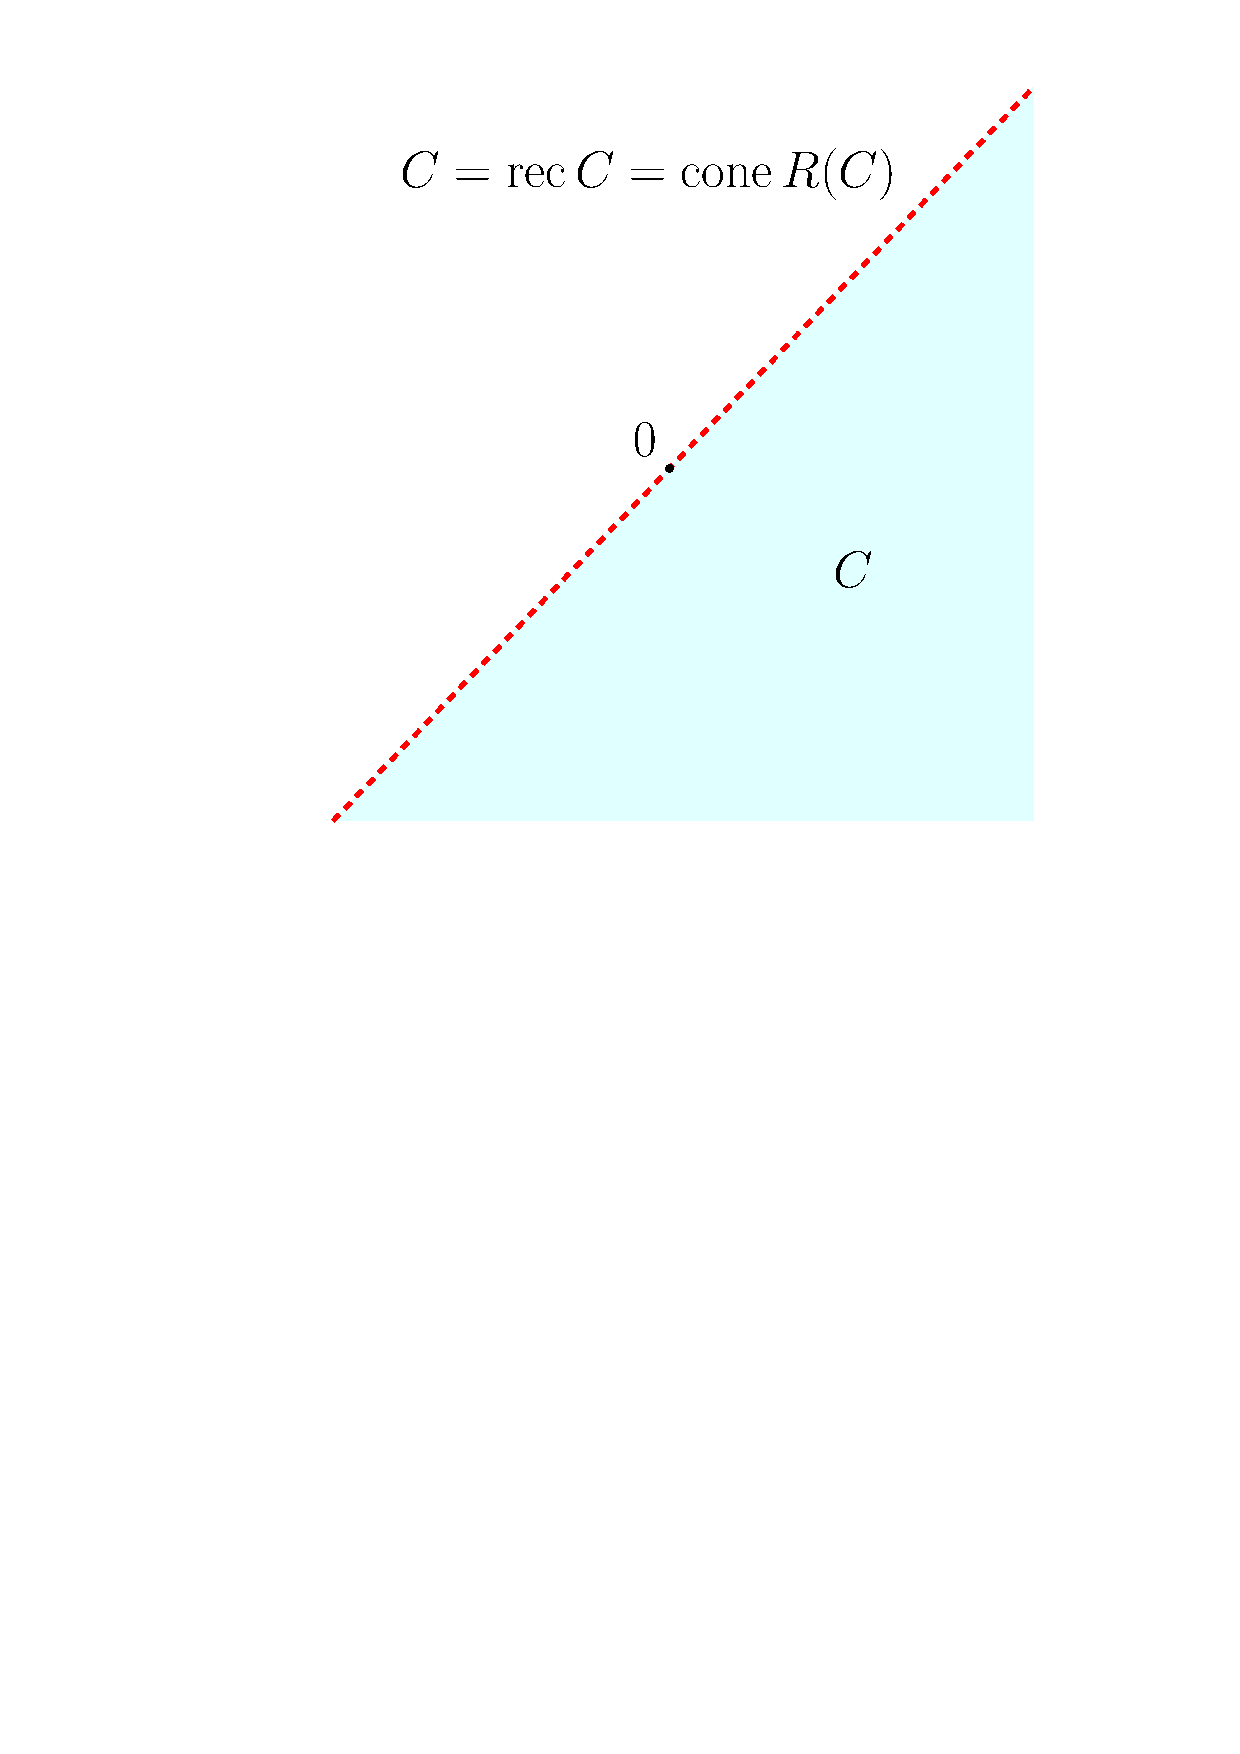
\includegraphics[scale=0.5]{figures/1697549641}
      \caption{Example of a non-pointed \( C \) not satisfying \( (3) \)}
    \end{subfigure}%
    \begin{subfigure}{.5\textwidth}
      \centering
     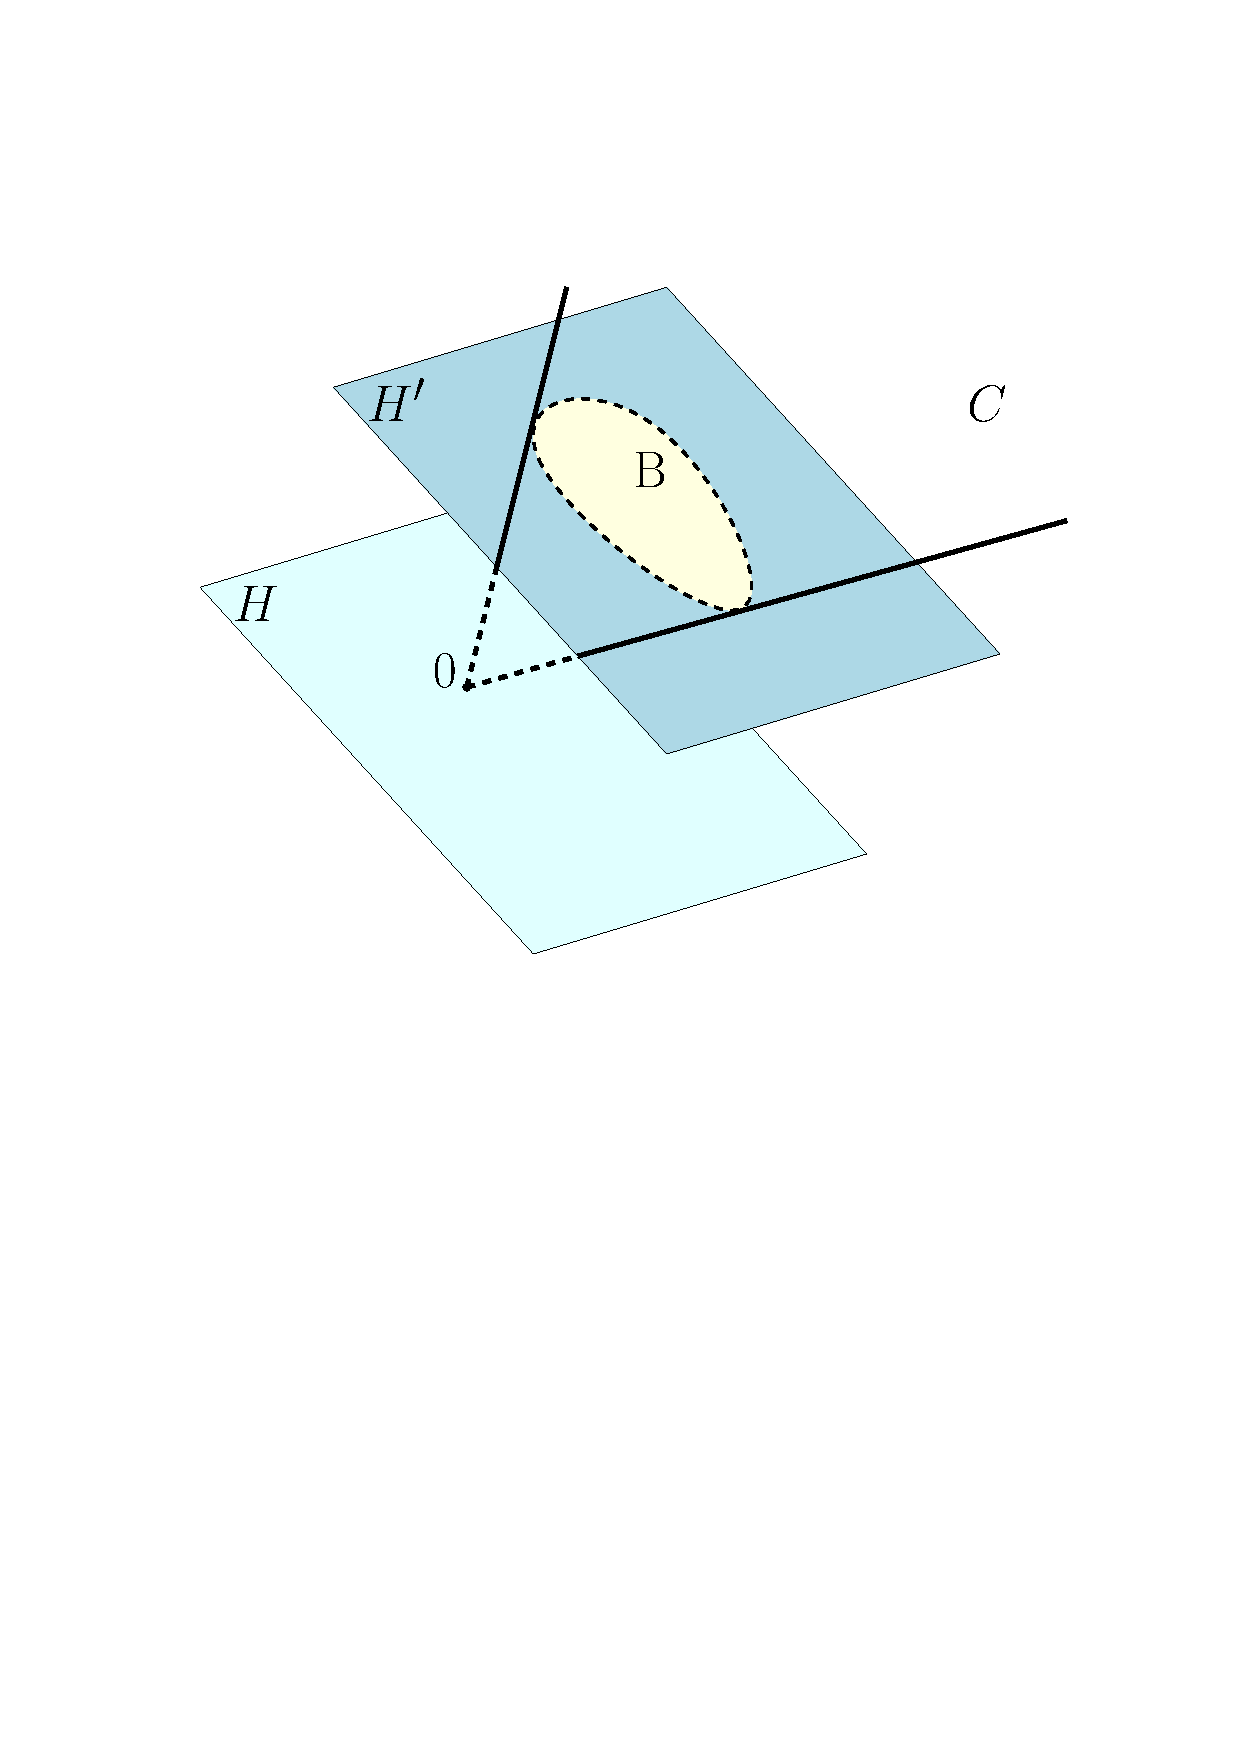
\includegraphics[scale=0.5]{figures/1697550459} 
      \caption{Illustration for the proof of \( (3) \)}
    \end{subfigure}
  \end{figure}
\end{proof}

% subsection Decomposition Theorem (end)

\subsection{Convex polyhedra} % (fold)
\label{sub:Convex polyhedra}

\begin{definition}
  A \textbf{convex polyhedron} (plural \textit{convex polyhedra}) \( P \) is
  the intersection of finitely many closed half-spaces.

  A \textbf{convex polytope} is a bounded convex polyhedron.
\end{definition}

An alternative definition for convex polyhedra is the result of the following
theorem.

\begin{theorem}[Alternative definition of convex polyhedra]
\label{thr:Alternative definition of convex polyhedra}
  If \( P \) is a convex polyhedra, then \( P = \operatorname{conv} E(\hat{P}) +
  \operatorname{cone} R(\hat{P}) + \operatorname{lin} P\), with \( \hat{P} = P
  \cap (\operatorname{lin} P)^{\perp } \).

  If \( P = \operatorname{conv} E + \operatorname{cone} R + L \), with \( L \)
  being a linear space, \( E \) and \( R \) are finite subsets of \(
  \mathbb{R}^{n} \), then \( P \) is a convex polyhedra.
\end{theorem}

\begin{proof}
  The first statement comes from Theorem \ref{thr:Decomposition Theorem}.

  To prove the second statement, consider \( \hat{P} = P \cap L^{\perp } \). It
  suffices to show that \( \hat{P} = \operatorname{conv} E + \operatorname{cone}
  R\), i.e. proving the statement for pointed \( P \).

  Now, consider the \( (n+1) \)-dimensional convex cone \( C \) defined as:
  \[
    C = \operatorname{cone} \left( \left\{ \begin{bmatrix} e \\ 1 \end{bmatrix},
    e \in E\right\} \cup \left\{ \begin{bmatrix} d \\ 0 \end{bmatrix}, d \in R \right\}  \right)   
  ,\], then we see that \( P \times \{1\} = C \cap H   \), with \( H: x^{n+1} =
  1\). The statement is now equivalent to the case \( P = C \) is a convex cone.
\end{proof}


Then, one can write \( P \) as \( P = \{x, Ax \ge  b\}   \) for some matrix \( A
\) and row vector \( b \), with the closed half-spaces defining \( P \) being
the half-spaces \( H_{i}: A^{i}x \ge  b^{i} \), i.e. for the case \( E = \{0\}
\).

Now, we need to prove the theorem for the \( E = L = \{0\}    \) case. Since \(
P = \operatorname{cone} R\), denote \( A \) as the matrix with columns being
elements of \( R \), then \( P = \{ Ax, x \ge  0\}   \). One can use
the \textbf{Fourier-Motzkin elimination method} to turn this form into \( P = \{x,
A'x \le b'\}   \).

\begin{quote}
  Here is a simple elimination method recursively eliminates the variables \( x^{1}, x^  {2},  \ldots , x^{n} \) from this linear system of equations:
  \begin{equation*}
  \begin{cases}
    y = Ax, A \in \mathbb{R}^{m\times n} \\
    x \ge  0
  \end{cases}
  \end{equation*}

  Denoting \( I = 1..(n-1), J = \{j, A^{j}_{n} = 0\}, J' = 1..m \setminus J
  \), we have:
  \begin{equation*}
  \begin{cases}
    y^{j} = A^{j}_{I}x^{I}, \forall  j \in J \\
    y^{j'} = A^{j'}_{I}x^{I} + A^{j'}_{n}x^{n}, \forall  j' \in J' \\
    x^{I} \ge  0 \\
    x^{n} \ge 0
  \end{cases}
  \end{equation*}

  This is equivalent to
  \begin{equation*}
  \begin{cases}
    y^{j} = A^{j}_{I}x^{I}, \forall  j \in J \\
    x^{n} = \frac{1}{A^{j'}_{n}}(y^{j'} - A^{j'}_{I}x^{I}), \forall  j' \in J'\\
    x^{I} \ge  0 \\
    x^{n} \ge 0
  \end{cases}
  \end{equation*}

  It is trivial to eliminate \( x^{n} \) from this system.
\end{quote}

\subsubsection{Extreme points and extreme directions of convex polyhedra} % (fold)
\label{sec:Extreme points and extreme directions of convex polyhedra}

Now, we will take a closer look at the extreme points of a convex polyhedron \(
P\).

\begin{definition}[Tight constraints]
\label{def:Tight constraints}
Let \( P: Ax \le  b \) be a convex polyhedron and \( x \in P \). Then, the set
\[
  \mathbb{I}(x) = \{i \in 1..m, A^{i}x = b^{i}\}  
.\] is called the \textbf{set of tight constraints indices at \( x \)}

In other words, \( \mathbb{I}(x) \) is the maximal multi-index such that \(
A^{I}x = b^{I} \).
\end{definition}

We also denote \( \mathbb{I}(F) \) as the intersection of all \( \mathbb{I}(x), x \in F
\). This will be useful when we look at the tight constraints of faces.

\begin{theorem}
\label{thr:Extreme point of convex polyhedra and matrix rank}
  Let \( P: Ax \le  b, x \in \mathbb{R}^{n} \) be a convex polyhedron.
  Then, \( x \) is an extreme
  point of \( P \) if \( \operatorname{rank} A^{\mathbb{I}(x)} = n \)
\end{theorem}

\begin{proof}
  Denote \( I = \mathbb{I}(x), I^{c} = 1..m \setminus I \).
  Then we can rewrite the conditions of \( x \) into \( A^{I}x = B^{I} \) and \(
  A^{I'}x < B^{I'}\).

  Now, if \( x \) is a convex combination of \( y \) and \( z \) with weight \(
  0 < \lambda < 1\), then 
  \begin{align*}
    b &= A^{I}x\\
      &= A^{I} \operatorname{lerp}(y, z, \lambda)\\
      &= \operatorname{lerp}(A^{I}y, A^{I}z, \lambda)\\
      &\le \operatorname{lerp}(A^{I}x, A^{I}x, \lambda) = A^{I}x = b
  .\end{align*}

  Since \( 0 < \lambda < 1 \), equality only happen when \( A^{I}y = A^{I}z =
  A^{I}x = b \). Hence, if \( \operatorname{rank} A^{I} = n \), the matrix \(
  A^{I} \) is invertible, thus leading to \( y = z = x =(A^{I})^{-1} b \),
  therefore \( x \) is an extreme point of \( P \).

  In the other case, \( \operatorname{rank} A < n \), then there exists \( u \)
  such that \( A^{I}u = 0 \). Consider \( y(\lambda) = x +\lambda u \), then 
  we need to find \( \lambda_{1} > 0 > \lambda_{2} \) such that \(
  y(\lambda_{1}), y(\lambda_{2}) \in P \) and since \( x \) is a strictly convex
  combination of \( y(\lambda_{1}) \) and \( y_{\lambda_{2}} \), \( x \) could
  not be an extreme point.

  Since \( A^{I}y(\lambda) = b^{I} \), we just need \( A^{I^{c}}y(\lambda) \le
  b^{I^{c}} \) to make \( y(\lambda) \in P \). This is trivial since the mapping
  \( f(\lambda) = A^{I^{c}}y(\lambda) \) is linear (and therefore continuous),
  and \( f(0) = A^{I^{c}} x < b^{I^{c}} \).

  Specifically, any \( \lambda \) satisfying \( |\lambda| < \varepsilon \), with
  \( \varepsilon > 0 \) defined as
  \[
    \varepsilon = \min_{\substack{j \in 1..m\\ A^{j}u \neq 0}} \left\{   \frac{b^{j} - A^{j}x}{|A^{j}u|}
  \right\}  
  .\] 
\end{proof}

\begin{corollary}
\label{cor:Finiteness of extreme points in convex polyhedra}
  All convex polyhedra \( P \subseteq \mathbb{R}^{n} \) has finitely many
  extreme points.
\end{corollary}

This is due to the fact that every extreme point of \( P \) corresponds to a set
of tight constraints indices \( \mathbb{I}(x) \), and since there can only be
finitely many such sets (not mentioning the full rank condition), there could
be only finitely many extreme points. An important thing to note is that, the
correspondence between \( x \) and \( \mathbb{I}(x) \) is one-to-one, with \( x
= \left(  A^{\mathbb{I}(x)} \right)^{-1}b\).

Similarly, we also have these analogous results for extreme directions.

\begin{definition}
\label{def:Polyhedral cone}
  A \textbf{polyhedral cone} is a cone that is also a convex polyhedra.
\end{definition}

\begin{theorem}
\label{thr:Recession cone of a convex polyhedra is polyhedral}
  The recession cone of a convex polyhedra \( P: Ax \le  b \) is a polyhedral
  cone \( C: Ax \le 0 \).
\end{theorem}

\begin{theorem}
\label{thr:Extreme directions of convex polyhedra and matrix rank}
  Let \( P: Ax \le  b, d \in \mathbb{R}^{n} \) be a convex polyhedron.
  Then, \( d \) is an extreme
  ray of \( P \) if \( \operatorname{rank} A^{\mathbb{I}(d)} = n - 1 \)
\end{theorem}

\begin{proof}
  By the rank-nullity theorem, \( A^{\mathbb{I}(d)} \) has rank \( n - 1 \) is
  analogous with the fact that the kernel of \( A^{\mathbb{I}(d)} \) is
  one-dimensional. Then, if \( d \) is a convex conical combination of \( d_{1}
  \) and \( d_{2} \), then \( d_{1} \) and \( d_{2} \) are both in this kernel,
  thus making the three vectors \( d_{1} \), \( d_{2} \) and \( d \) lies on the
  same line, which means that \( d \) is an extreme direction.

  The other direction could also be proven similarly to the proof of Theorem
  \ref{thr:Extreme point of convex polyhedra and matrix rank}, by considering
  some vector \(
  u\) linearly independent from \( d \) such that \( A^{\mathbb{I}(d)} = 0 \)
  and consider the function \( d(\lambda) = d + \lambda u \).
\end{proof}

% subsubsection Extreme points and extreme directions of convex polyhedra (end)
\iffalse
\subsubsection{Polar and the Minkowski-Weyl's Theorem} % (fold)
\label{sec:Polar and the Minkowski-Weyl's Theorem}

\begin{definition}[Polar]
\label{def:Polar}
  Let \( V \) be a vector space and \( X \subseteq V \). Then,
  \( X^{\circ} \), called the \textbf{transposed polar} of \( X \), is defined as:
  \[
    X^{\ostar} = \{y \in V^{\star}, yx \le 1, \forall x \in X \}  
  .\], with \( V^{\star} \) denoting the \textbf{dual space} of \( V \).

  If \( V = \mathbb{R}^{n} \) then\footnote{This is an abuse of notation, \(
  V^{\star} \) is supposed to be a set of linear functionals, not matrices.
Also, we will abuse the notation even more, by considering the double dual of a
vector space the same thing as the original vector space (the two spaces are
naturally isomorphic.)}
  \( V^{\star} = \mathbb{R}^{1\times n} \) and
  vice versa, then the \textbf{transpose} operation can be used to convert
  between \( V \) and \( V^{\star} \). Then,
  the transpose of \( X^{\ostar} \) is called the \textbf{polar} of \( X \):
  \[
    X^{\circ} = (X^{\ostar})^{T} = \{x^{T}, x \in X^{\ostar}\}   
  .\] 
\end{definition}

Then, one can see that the polar of a linear space is its orthogonal complement,
For convex cones, the transposed polar can be redefined to \( X^{\circ} = \{y \in
\mathcal{L}(X), yx \le  0, x \in X\}   \).

The polar of an arbitrary (Euclidean) set is a closed and convex set.
since it could be written as intersection of (infinitely many) closed and convex
half-spaces:
\[
  X^{\circ} = \bigcap_{x \in X} \{y \in \mathbb{R}^{n}, y^{T}x \le  1\}  
.\] 

The polar operation can also be applied twice to a set \( X \), resulting in the
set \( (X^{\circ})^{\circ} \), which is not necessarily to be \( X \). In
particular, we have
\[
  (X^{\circ})^{\circ} = \overline{\operatorname{conv} (X \cup  \{0\}  )} 
.\] 

\begin{proof}
  Denote \( X' = (X^{\circ})^{\circ} \), then it is trivial that \( 0 \in X' \)
  and \( X \subseteq X' \). Since \( X' \) is closed and convex, the set \( X''
  = \overline{\operatorname{conv} \{X \cup \{0\}  \}  } \subseteq X' \). Now, we
  just need to prove equality.

  Take \( y \in X''^{c} \), we will prove \( y \in X'^{c} \), which will be what
  we needed. This is equivalent to finding \( z \in X^{\circ} \) such that \( yz
  > 1\). Using Theorem \ref{thr:Hyperplane Separation Theorem}, we find \( H: ax
  = \alpha\) that separates \( \{y\}   \) and \( X'' \), i.e. \( ay > \alpha
  \ge ax, \forall x \in X'' \). Since \( 0 \in X'' \), we have \( \alpha \ge  0
  \).

  If \( \alpha > 0 \), then let \( z = \frac{1}{\alpha} a \), we have \( zx \le 1,
  \forall x \in X\), which means \( z \in X^{\ostar} \). Then, \( zy > 1 \),
  which is a contradiction.

  If \( \alpha = 0 \), then let \( \varepsilon = ay > 0 \), then \( z =
  \frac{2}{\varepsilon}a \) satisfies \( zx \le  1 < 2 = zy, \forall x \in X \),
  which is another contradiction.

  Hence, \( y \) does not exist, and \( X' = X'' \).
\end{proof}
\fi
\iffalse
\subsubsection{Minkowski-Weyl's Theorem} % (fold)
\label{sec:Minkowski-Weyl's Theorem}
Minkowski-Weyl's TheoremAn important property of convex polyhedra is the following theorem.

\begin{theorem}[Minkowski-Weyl's Theorem]
\label{thr:Minkowski-Weyl's Theorem}
  Denote \( \operatorname{conv} V \) as the \textbf{convex hull} of \( V \), \(
  \operatorname{cone} R\) as the convex cone generated by \( R \), \( E(P) \)
  and \( R(P) \) as the set of all extreme points and extreme directions of \( P
  \), respectively. Then
  \begin{itemize}
  \item \textbf{Minkowski's Theorem:}
  \( P \) is a convex polyhedron then
  \( P = \operatorname{conv} E(P) + \operatorname{cone} R(P) \),
  with \( E(P) \) and \( R(P) \) denoting the set of all extreme points and
  extreme directions of \( P \), respectively.
\item \textbf{Weyl's Theorem:}
  If there exists finite sets \( E(P), R(P)  \) such that \( P = \operatorname{conv}
  E(P) + \operatorname{cone} R(P)\), then \( P \) is a convex polyhedron.
  \end{itemize}
\end{theorem}

\begin{proof}
  To prove this theorem, we will try to reduce this problem to the \( b = 0 \)
  case. This case would be proven separately in Theorem
  \ref{thr:Minkowski-Weyl's
  Theorem for Convex Cones}.

  \begin{itemize}
  \item \textbf{Minkowski's Theorem}: Let \( P: Ax \le  b, x \in \mathbb{R}^{n}
    \) Consider the following matrices and
    vectors:
\begin{align*}
  x' &= \begin{bmatrix} x \\ 1 \end{bmatrix} \in \mathbb{R}^{n+1} \\
  A' &= \begin{bmatrix} A & -b \\ -\mathbf{e_{n+1}}^{T} & 0 \end{bmatrix}
  \in \mathbb{R}^{(n + 1) \times  (m + 1)}
\end{align*} (\( \mathbf{e_{n+1}} \) is the \( (n+1) \)-th standard basis
(column) vector).

Then \( Ax \ge b \) if and only if \( A'x' \ge  0 \).

Hence, we will consider the \( (n+1) \)-dimensional polyhedral cone \( C: A'x'
\le  0, x' \in \mathbb{R}^{n+1} \). By Theorem \ref{thr:Minkowski-Weyl's Theorem
for Convex Cones}, \( C = \operatorname{cone} R(C)
\).

    Now take an arbitrary extreme direction \( d' \) of \( C \)
    \[
      d' = \begin{bmatrix} d & z \end{bmatrix} \in \mathbb{R}^{n+1}, \text{ for
      some } d \in \mathbb{R}^{n}, z \in \mathbb{R}
    .\] 

    We have \( A'd' \ge  0 \), which is equivalent to \( Ad - bz \le  0 \) and
    \( z \ge  0 \)

    If \( z = 0 \), then \( Ad \le  b \), which means that \( d \) is an
    recession direction of \( P \). If \( d = \operatorname{lerp}(d_{1}, d_{2},
    \lambda) \) for some \( \lambda \in (0, 1) \) and recession direction \(
    d_{1} \) and \( d_{2} \), we can see that \( d' =
    \operatorname{lerp}(d_{1}', d_{2}', \lambda) \), with \( d'_{i} =
        \begin{bmatrix} d_{i} & 0 \end{bmatrix}^{T}  \), which is a
        contradiction to the fact that \( d' \) is an extreme direction.
    
    If \( z > 0 \), then let \( v = \frac{1}{z} d \), then \( Av \le  b \),
    following a similar logic, we deduce that \( v \) is an extreme point of \(
    P\).

    Denote \( d_{i}' = \begin{bmatrix} d_{i} & z_{i} \end{bmatrix}  \) as
    the \( i \)-th extreme direction of \( C \). Let \( I = \{i, z_{i} > 0\}
    \) and \( I^{c} = \{i, z_{i}  = 0\}   \),
    then \( x' = \begin{bmatrix} x
    & 1\end{bmatrix}  \in C =
    \operatorname{cone} R(C) \) iff there exists \( \lambda \ge 0 \) such that:
    \begin{align*}
      x' &= d_{i}'\lambda^{i}\\
      &= d'_{I}\lambda^{I} + d'_{I^{c}}\lambda^{I^{c}}
    .\end{align*}

    Separating the first \( n \) coordinates and the \( (n+1) \)-th one, we have
    \begin{align*}
      x &= d_{I}\lambda^{I} + d_{I^{c}}\lambda^{I^{c}} \\
      1 &= z_{I}\lambda^{I}
    .\end{align*}

    Substituting \( v_{i} = \frac{1}{z_{i}}d_{i} \in E(P) \), we have
    \begin{align*}
      x &= v_{I}z_{I}\lambda^{I} + d_{I^{c}}\lambda^{I^{c}}\\
      1 &= z_{I}\lambda^{I}
    .\end{align*}

    Finally, denoting \( w_{i} = z_{i}\lambda^{i} \), from the second identity,
    we have the sum of all components of \( w \) is 1, and therefore, we can
    write the above
    expression as \( x = \mathcal{C}(v_{I}, w_{I}) + \mathfrak{C}(d_{I^{c}},
    \lambda^{I^{c}}) \), we have written \( x \) as the sum of a convex
    combination of extreme points \( v_{I} \) and a convex conical combination
    of extreme directions \( d_{I^{c}} \). To prove the other direction, one
    can simply repeat the above logic, but in reverse.

  \item \textbf{Weyl's Theorem:}
    Following the intuition of the above proof, we will consider the set
    \( C = \operatorname{cone} R(C) \), with finite \( R(C) \) given by:
    \begin{align*}
      R(C) &= \left\{ \begin{bmatrix} v \\ 1 \end{bmatrix} , v \in E(P) \right\}
      \cup \left\{ \begin{bmatrix} d \\ 0 \end{bmatrix} , d \in R(P) \right\}  \\
    .\end{align*}
    Then, \( C \) is a polyhedral cone with constraints \( A'x' \le  0 \).
    Assuming
    \begin{align*}
      A' = \begin{bmatrix} A & -b \end{bmatrix}, A \in \mathbb{R}^{(n + 1)
      \times  m}
    ,\end{align*}we have \( P = \{x \in \mathbb{R}^{n}, Ax \le  b\}   \)
  \end{itemize}
\end{proof}

Now, all that's left is to prove Minkowski-Weyl's Theorem for convex cones.

\begin{theorem}[Minkowski-Weyl's Theorem for Convex Cones]
\label{thr:Minkowski-Weyl's Theorem for Convex Cones}
  Let \( P \subseteq \mathbb{R}^{n} \), then the following statements are
  equivalent:

  \begin{enumerate}
  \item \( P \) is a polyhedral cone, i.e. there exists \( A \in \mathbb{R}^{m
    \times  n} \) such that \( P = \{x \in \mathbb{R}^{n}, Ax \le  0\}   \)
  \item \( P \) is a \textit{finitely generated cone}, i.e. there is some matrix
    \( R \) such that \( P = \{x, x = R\lambda, \lambda \ge  0\}   \)
  \end{enumerate}
\end{theorem}

\begin{proof}
  The "\( (2) \implies (1) \)" direction is trivial. One can apply
  Fourier-Motzkin elimination to the linear system of inequalities \( x =
  R\lambda, \lambda \ge 0 \) to eliminate the variables \( \lambda^{1},
  \lambda^{2}, \ldots , \lambda^{k} \) from the system, leaving a system of
  inequalities in the form of \( Ax \le 0 \). Note that no constants were
  generated in the process, hence the \( 0 \) on the RHS.

  Before proceeding, we will introduce a new concept:

  We say that \( (A, R) \) is a \textit{double description pair} (DDP) if
  \( Ax \le  0 \iff \exists \lambda \ge 0, x = R\lambda  \). Then, we will
  proceed to prove that \( (R^{T}, A^{T}) \) is also a DDP.
  \begin{align*}
    &R^{T}y \le 0\\
    &\iff \lambda^{T} R^{T} y \ge 0, \forall  \lambda \ge 0\\
    &\iff (R\lambda)^{T} y \ge 0, \forall  \lambda \ge 0
  .\end{align*}
  Let \( x = R\lambda \), then \( R^{T}y \le 0 \) iff \( x^{T}y \ge 0, \forall
  \lambda \ge 0, x = R\lambda \), or equivalently \( Ax \le  0 \). Then, the
  last statement is equivalent to the statement: \( Ax \le  0 \implies x^{T}y \le  0 \)

  To conclude this proof, we need to use \textbf{Farkas' Lemma}.

  \begin{lemma}[Farkas' Lemma]
  \label{farkas}
    \( ax \ge  0, \forall  x \) s.t. \( Ax \ge  0 \) iff \( a = yA \) for some
    row vector \( y \ge  0 \)
  \end{lemma}

  \begin{proof}[Proof of Farkas' lemma]
    If \( a = yA \), then \( ax = yAx \ge  0, \forall  Ax \ge 0 \).

    If \( ax \ge  0, \forall Ax \ge 0 \) and \( a \neq  yA, \forall  y\ge 0 \),
    then consider the set \( S = \{yA, y \ge 0\}   \). Since \( a \notin S \)
    and \( S \) is closed, using Theorem \ref{thr:hst-closed-pt}, there is a
    hyperplane \( H \) strictly separating \( S^{T} \) and \( \{ a^{T}\}   \).
    Assuming \( H = \{t, x^{T}t \ge  \alpha\}   \) satisfies \( ax  <  \alpha
    \le   \inf Sx \). Note that \( 0 \in Sx \), then \( \alpha \) must be
    non-positive. If \( \alpha < 0 \) and the hyperplane \( H' = \{ t, x^{T}t =
    0\}   \) could not separate the two sets, then there exists some \( t \in S
    \) such that \( tx < 0 \). Then, there exists \( k > 0 \) such that \( t(kx)
    < \alpha\), with \( kx \in S \), which means the original hyperplane also could
    not separate the two sets, which is a contradiction. Hence, the hyperplane
    \( H' \) could separate the two set, i.e. \( ax < 0 \le \inf Sx \). Then,
    we have \( A_{i}x \ge  0 \) for all \( i \), since \( A_{i} =
    A\mathbf{e_{i}} \in S \), with \( \mathbf{e_{i}} \) denoting the \( i \)-th
    standard basis vector, and hence \( Ax \ge 0 \). To conclude, \( ax < 0 \)
    for some \( x \) s.t. \( Ax \ge 0 \), which is another contradiction.
  \end{proof}

Continuing with the proof, we have
\begin{align*}
  &(Ax \le 0 \implies x^{T}y \le 0)\\
  &\iff(Az \ge  0 \implies z^{T}y \ge  0) \text{ (letting \( z = -x \))}\\
  &\iff \exists \lambda \ge 0,  y = \lambda A\\
  &\iff \exists  \lambda' = \lambda^{T} \ge 0, y^{T} = A^{T}\lambda'
.\end{align*}

Hence \( (R^{T}, A^{T}) \) is a DDP.

So to find \( R \), one find do Fourier-Motzkin on \( A^{T} \) to get \( R^{T}
\). Now that \( R \) exists, we have \( C = \{x, Ax \ge 0\} = \{x, \exists
\lambda \ge 0, x = -R\lambda\}  \)

Now, we will prove that \( -R_{i} \) are recession directions of \( C \).
Since \( R_{i} = R\mathbf{e_{i}}, \mathbf{e_{i}} \ge 0 \), \( R_{i} \in P \),
and \( AR_{i} \ge  0 \). Then, for every \( x \in P, t \ge 0 \), we have \( A(x
- tR_{i}) = Ax - tAR_{i} \le  0 \), which means that \( R_{i} \) is a recession
direction of \( C \). Pick columns from \( R \) to form a conical basis of \( R \)'s
column space, then this basis is able to span the recession cone of \( C \), due
to every recession direction \( d \) of \( C \) can be written as \( d =
R\lambda = R'\lambda' \) with some \( \lambda, \lambda' \ge  0 \).
\end{proof}

% subsubsection Minkowski-Weyl's Theorem (end)
\fi
\subsubsection{Faces of convex polyhedra} % (fold)
\label{sec:Faces of convex polyhedra}

\begin{theorem}
\label{thr:Basic properties of faces}
Faces of convex polyhedra are convex polyhedra.
\end{theorem}

\begin{proof}
  Let \( P \) be a convex polyhedron, then by Theorem \ref{thr:Alternative
  definition of convex polyhedra}, if \( \hat{P} = P \cap (\operatorname{lin}
  P)^{\perp } \), \( P = \operatorname{conv} E(\hat{P}) + \operatorname{cone}
  R(\hat{P}) + \operatorname{lin} P \).

  Let \( F \) be a face of \( P \), then
  by Theorem \ref{thr:Decomposition Theorem}, \( F =
  \operatorname{conv} E(F) + \operatorname{cone} R(F) + \operatorname{lin} F \).

  Since \( E(F) \subseteq E(P) \) is finite, it suffices to show that \( R(F) \)
  is also finite. In actuality, \( R(F) \subseteq R(P) \), which is finite, so
  that validates our claim.

  To prove \( R(F) \subseteq R(P) \), assuming \( \exists d \in R(F) \setminus
  R(P) \). Then, there exists \( d_{1}, d_{2} \in \operatorname{rec} P \) such
  that \( d = \mu d_{1} + \nu d_{2} \), with \( \lambda, \mu > 0\) and \(
  d_{1} \) and \( d_{2} \) not parallel.

  Let \( x_{0} \in F \) and consider \( x = x_{0} + \lambda d, x_{1} = x_{0} +
  \lambda_{1} d_{1}, x_{2} = x_{0} + \lambda_{2}d_{2} \). To make \( x, x_{1},
  x_{2} \) collinear, we pick \( \lambda_{1}, \lambda_{2} > 0 \) as
  such:

  \begin{align*}
    x &= \operatorname{lerp}(x_{1}, x_{2}, t) \\
    \lambda d &= \operatorname{lerp}(\lambda_{1}d_{1}, \lambda_{2}d_{2}, t)
  .\end{align*}

  Letting \( \lambda_{1} = \lambda_{2} \), we have:
  \begin{align*}
    \lambda d &= \lambda_{1}\operatorname{lerp}(d_{1}, d_{2}, t) \\
              \lambda(\mu + \nu)d &= \lambda_{1} (t d_{1} + (1-t)d_{2}) \\
              \implies \lambda \mu &= t\lambda_{1} , \lambda \nu =
              (1-t)\lambda_{1} \\
              \implies \lambda &= \frac{\lambda_{1}}{\mu + \nu}
  .\end{align*}

  Since \( x \) is a strict linear combination of \( x_{1} \) and \( x_{2}
  \), both \( x_{1} \) and \( x_{2} \) must lie on \( F \), thus making \(
  d_{1} \) and \( d_{2} \) extreme directions of \( F \). This contradicts with
  the fact that \( d \) is an extreme direction of \( F \).
\end{proof}

Using this seemingly trivial properties of polyhedral faces, we have the
following theorem.

\begin{theorem}[Face Representation Theorem]
\label{thr:Face Representation Theorem}
  Let \( P \subseteq \mathbb{R}^{n} \) be a convex polyhedron and \( F \subseteq
  P \), then, the following statements are equivalent:

  \begin{enumerate}
    \item \( F \) is a face of \( P \).
    \item \( F \) is an exposed face of \( P \).
    \item There exists multi-index \( I \subseteq 1..m \) such that \( F = \{x
      \in P, A^{I}x = b^{I}\}   \).
  \end{enumerate}
\end{theorem}

\begin{proof}
  \( (3) \implies (1) \) is trivial.

  To prove \( (1) \implies (2) \), let \( x_{0} \in \operatorname{ri} F \). By
  Lemma \ref{lem:Points on relative boundary lies on a proper face}, \( x_{0} \in
  \operatorname{relbd} P \). Let \( H \) be the supporting hyperplane of \( P \)
  at \( x_{0} \), and denote \( G = P \cap H \).

  \begin{quote}
    Assuming \( P \subseteq H_{0}^{-}: ux <\gamma \), we can trivially see that \(
    ux \le \gamma, \forall  x \in E(P) \) \( ud \le 0, \forall d \in R(P) \) and
    \( ul = 0, \forall  l \in \operatorname{lin} P \).

    Since \( x_{0} \in \operatorname{ri} F \), one can write \( x_{0} =
    \mathcal{C}(E(F), \lambda) + \mathfrak{C}(R(F), \mu) + l \) with some \(
    \lambda, \mu > 0, l \in \operatorname{lin} F \subseteq \operatorname{lin} P
    \). The strict inequality in \( \lambda, \mu > 0 \) comes from \( x_{0} \in
    \operatorname{ri} F\) (if one want to avoid proving this, one can pick \(
    \lambda, \mu > 0 \) and then define \( x_{0} \) using the above identity).

    Then, we have \( u\mathcal{C}(E(F), \lambda) = \mathcal{C}(uE(F), \lambda)
    \le \gamma \) since \( E(F) \subseteq P \). Similarly, we have \(
    u\mathfrak{C}(R(F), \mu) \le 0 \) and \( ul = 0 \), which means \( ux_{0} \le
    \gamma \). Since equality happens and all weights are positive, every
    inequality above must have equality, i.e. \( ue = \gamma, ud = 0, \forall  e
    \in E(F), d \in R(F)\). Using Theorem \ref{thr:Decomposition Theorem}, one
    can trivially prove that \( F \subseteq H_{0}: ux = \gamma \).
  \end{quote}

  Since \( F \subseteq H \), \( F \subseteq G \).
  Let \( G' \) be the minimal exposed face of \( P \) that contains \( F \),
  induced by the hyperplane \( H: ax = \alpha \). WLOG, assuming \( 
  P\subseteq H^{-}: ax \le  \alpha \).

  We will prove that \( F = G' \). Assuming that this
  is not the case, \( F \) is a proper face of \( G' \) and \( x \in
  \operatorname{relbd} G' \). Therefore, there exists \( H': bx = \beta \),
  the supporting hyperplane of \( G' \) at \( x \). WLOG, assuming \( G'
  \subseteq H'^{-}: bx \le \beta \). Furthermore, using Lemma
  \ref{lem:Supporting Hyperplane Theorem (Stronger variant)}, we can find an \(
  y \in G'\) such that \( by < \beta \). Using similar reasoning as above, we
  also have \( F \subseteq H' \).

  Then, \( \forall x \in G', ax \le \alpha, bx \le \beta \), and \( \forall x
  \in F, ax = \alpha, bx = \beta \). Consider the
  set \(
  X_{\lambda} = \{x \in P, (\lambda a + b)x = \lambda \alpha + \beta\}  \) for
  some \(  \lambda > 0 \). We trivially have \( F \subseteq X_{\lambda}
  \subsetneq G' \) (since \( y \in G' \) and \( y \notin X_{\lambda} \)), so to
  have a contradiction, we need to pick some \( \lambda > 0 \) such that \(
  X_{\lambda} \) is an exposed face of \( P \), i.e. find \( \lambda > 0 \) s.t.
  \( (\lambda a + b)x \le \lambda\alpha + \beta \) for every \( x \in P \).

  Rewrite the inequalities into \( \lambda(ax
  -\alpha) + (bx - \beta) \le  0 \). For points \( x \in P \) with \( ax -
  \alpha < 0
  \), no matter what \( bx - \beta \) is, the inequality will hold for
  arbitrarily large \( \lambda \). For \( x \in P \) with \( ax - \alpha =0 \),
  we see that \( x \in G' \) and therefore \( bx - \beta \le  0 \), and the
  inequality still holds. Hence, there exists some large \( \lambda > 0 \) such
  that this inequality holds for every \( x \in P \). In particular, here is a
  value for \( \lambda \):
  \[
    \lambda > \max \left\{ 0, \max_{\substack{x\in E(P)\\ax<\alpha}} -\frac{bx
    - \beta}{\alpha - ax}, \max_{\substack{d \in R(P)\\ ad < 0}}
  \frac{bd}{-ad}\right\}
  .\]

  Hence, we got our contradiction, and \( F \) is an exposed face of \( P \).

  Finally, we will prove \( (3) \implies (1) \). Assuming that \( F = P \cap H
  \) with \( H: ax = \alpha \) and \( P \subseteq H^{-}: ax \le
  \alpha\), we will find the multi-index \( I \) s.t. \( F = \{x \in P, A^{I}x =
  b^{I}\}\).

  \( P \subseteq H^{-} \) suggests the inequality \( ax \le \alpha \) could be
  implied from constraints \( A^{i}x \le  b^{i} \), which suggests that \( ax
  \le \alpha \) could be a convex conical combination of such constraints, wrt some
  weight \( \lambda \ge 0 \). This
  actually holds true (by Lemma \ref{lem:Forms of valid inequalities}), and denote
  \( y = \lambda^{T} \), then \( y \in \mathbb{R}^{1\times n}, y \ge 0 \) such
  that \( a = yA \)  and \( \alpha = yb \).

  Consider \( x \in F \subseteq P \), we have \( ax = y_{I}A^{I}x = \alpha =
  y_{I}b^{I} \) or \( y_{I}(A^{I}x - b^{I}) = 0 \). Since \( y_{I} > 0 \) and \(
  A^{I}x - b^{I} \le 0\) for every \( x \in P \), we must have \( A^{I}x = b^{I}
  \), and we have \( F = \{x \in P, A^{I}x = b^{I}\}   \).
\end{proof}

\begin{corollary}
\label{cor:Finiteness of faces in convex polyhedra}
  All convex polyhedra \( P \subseteq \mathbb{R}^{n} \) has finitely many faces.
\end{corollary}

\begin{proof}
  Every face corresponds one-to-one to a multi-index \( I \), and there are only
  finitely many such \( I \). Hence, there must be finitely many faces of a
  given convex polyhedron. 
\end{proof}

% subsubsection Faces of convex polyhedra (end)

% subsection Convex polyhedra (end)

% section Convex polyhedra (end)

\section{Existence and properties of solutions of linear programs} % (fold)
\label{sec:Existence and properties of solutions of linear programs}

Firstly, since \( D = \{x\ge 0, Ax \ge  b\}   \) is a convex set (this can be
trivially seen due to the linearity of the convex combination operation) and \(
f(x)=cx\) is a convex (and a concave) function on \( \mathbb{R}^{n} \), then
every (S)LOS of the linear program is a (S)GOS.

The set \( D \) is already closed and \( f(x) \) is continuous, and hence
the problem will have a GOS if \( D \) is bounded.

Consider the set of GOSes for the minimization problem \( S =
\operatorname{Argmax} \{cx, Ax \le  b\}   \), we can see that this set is
actually a face of the convex polyhedra \( P: Ax \le b \). To prove this,
assuming \( x = \operatorname{larp}(y, z, \lambda) \), \( \lambda \in (0, 1) \)
with some \( y, z \in P \), we will see that \( b = Ax = \operatorname{lerp}(Ay, Az,
\lambda) \le  b \). Since \( \lambda \in (0,1) \), equality happens implies that
\( Ay = Az = b \) and therefore \( y, z \in S \).

If \( S \) is pointed, then \( S \) has at least an extreme point. This extreme
point is a GOS of the problem. Hence, if \( P: Ax \le  b \) is a pointed convex
polyhedron, then the problem will either has a GOS at a vertex of \( P \) or
simply does not have a GOS. Hence, in solving linear program, we usually only
need to look at the extreme points of \( P \). These points are also called
\textbf{extreme solutions}.

From this observation, we have this following algorithm to solve linear
programs.

\begin{python}
def solve_lp_naive(A, b, c):
  # retrieve dimension count
  m, n = dimensions(A)

  # keep track of best result
  best = Infinity
  best_sol = None

  # loop over vertices, using Theorem 3.2.15
  # note that here, if there are no invertible `I` (i.e. when m < n),
  # our problem don't have any extreme solutions
  for I in itertools.permutation(range(m), n):
    submatrix = A^I
    if not invertible(submatrix):
      continue
    # typically, we solve the linear system of equations directly
    # instead of inverting the matrix for performance reasons,
    # but for clarity, we will invert here
    x = invert(submatrix) * b
    fx = c * x

    if fx < best:
      best = fx
      best_sol = x
  return best, best_sol
\end{python}

The loop is ran \(\binom{m}{n}\) times, which is basically factorial
complexity, and in every iteration, we need to solve a linear system of
equations with \( n \) equations and \( n \) variables, which has the time
complexity of \( O(n^3 ) \), which makes this naive algorithm
unbearably slow when compared to the simplex method.

% section Existence and properties of solutions of linear programs (end)

\section{Geometric method of solving linear programs} % (fold)
\label{sec:Geometric method of solving linear programs}

Since \( f(x) = cx \) is linear, its level sets are parallel hyperplanes \( cx =
\alpha \), this allows us to easily visualize the complete space of level sets.

By translating the line by a vector \( v \), we got another level set \( cx =
\alpha - cv \). If \( cv < 0 \), for example when \( v = -c^{T} \), we ended up
with a set of more optimal solutions than the solutions in the original level
set.

Using this simple observation, we have the following method to solve linear
programs. This method is only meant to be used for humans, since it relies
heavily in visual and geometric sense, hence the name.

\begin{itemize}
\item Pick an arbitrary solution \( x_{0} \) of the problem and draw the level
  set \( cx = cx_{0} \).
\item Nudge this hyperplane in the \( c^{T} \) direction 
  until it barely touches the convex polyhedron \( P:
  Ax \le b\). If the process could go on forever, there are no GOSes.
\item The intersection of the nudged hyperplane and the convex polyhedron is the
  set of GOSes for the problem.
\end{itemize}

The nudging process, if done on a computer, is inefficient or even borderline
impossible, hence, this method can only be done visually. Moreover, since humans
could only visualize up to 3 dimensions, this method only works for \( n \le 3
\). However when \( n = 3 \) the process involves imagining 3D space, which could
be very hard to do without the help of graphing softwares, so this method is
typically used when \( n = 2 \).

% section Geometric method of solving linear programs (end)

\section{Simplex method} % (fold)
\label{sec:Simplex method}

\subsection{Geometric simplex method} % (fold)
\label{sub:Geometric simplex method}

The idea of the simplex method is that one starts at an extreme solution of the
linear program, and walk along an edge of the convex polytope that minimizes the
objective method the most.

\begin{python}
def solve_lp_simplex_geom(A, b, c, x0 = pick_extreme_sol_on_polyhedron(A, b)):
  best_decrement = Infinite
  best_x1 = None
 
  for edge in edges_from_extreme_sol_of_polyhedron(x0, A, b):
    if c * edge.direction() >= 0:
      continue
    if edge.is_infinite():
      return "No GOSes"
    else:
      _, x1 = edge.endpoints()
      decrement = c * (x1 - x0)
      if decrement < 0 and decrement < best_decrement:
        best_decrement = decrement
        best_x1 = x1
  
  if best_x1 is None:
    return x0
  else:
    return solve_lp_simplex_geom(A, b, c, x1)
\end{python}

This algorithm has a host of problems, but this is not how the general simplex
method works so we will not attempt to fix this thing. The algorithm here is
also very slow, since the act of finding edges for an extreme solution is not
straightforward and efficient.

% subsection Geometric simplex method (end)

\subsection{Extreme solutions of augmented form linear programs} % (fold)
\label{sub:Extreme solutions of augmented form linear programs}

Consider the following AFLP \( (P) \):
\begin{align*}
  \min\, &f(x) = cx\\
  \text{s.t.}\, &Ax = b, x \ge 0, x\in \mathbb{R}^{n},
\end{align*} with \( A \in \mathbb{R}^{m \times  n}, b \in \mathbb{R}^{n}, c \in
\mathbb{R}^{1\times  n}\).

From Theorem \ref{thr:Extreme point of convex polyhedra and matrix rank}, we see
that every extreme solution \( x_{0} \) of \( (P) \) corresponds to a
multi-index \( \mathbb{I}(x_{0}) \subseteq 1..(m + n) \) such that:
\[
  \operatorname{rank} \begin{bmatrix} A \\ -I_{n}
  \end{bmatrix}^{\mathbb{I}(x_{0})} = n
.\] 

Since the rank of a matrix is at most its lower dimension, we must have \( n \le
|\mathbb{I}(x_{0})|\). Here, there are two cases:

\begin{itemize}
  \item If \( |\mathbb{I}(x_{0})| = n \), then the matrix \( \begin{bmatrix} A
  \\ -I_{n} \end{bmatrix} ^{\mathbb{I}(x_{0})} \) has full rank, and we say that
  \( x_{0} \) is a \textbf{non-degenerate} extreme solution of \( (P) \).
\item Otherwise, \( |\mathbb{I}(x_{0})| > n \), we say that \( x_{0} \) is a
  \textbf{degenerate} extreme solution of \( (P) \).
\end{itemize}

Consider the set \( J(x_{0}) = \{j, x_{0}^{j} > 0 \}   \) and its complement \(
J^{c}(x_{0}) = \{j, x_{0}^{j} = 0\}  \). In other words, \( J^{c}(x_{0}) \) is
the set of indices to the constraints \( x^{j} \ge 0 \) that \( x_{0} \) is
tighted at, and therefore \( J^{c}(x_{0}) \subseteq \mathbb{I}(x_{0}) \).

The set \( J(x_{0}) \) is called the set of \textbf{basic indices} of the
extreme solution \( x_{0} \), and \( J^{c}(x_{0}) \) is called the set of
\textbf{non-basic indices} of \( x_{0} \).

However, for AFLPs, there is another way to indicate whether a solution \( x_{0}
\) is an extreme solution or not.

\begin{theorem}
\label{thr:Linear independent condition of basic columns for extreme solutions}
  Let \( x_{0} \) be a solution of \( (P) \), and denote \( J(x_{0}) = \{j,
  x_{0}^{j} > 0\}   \). Then \( x_{0} \) is an extreme solution of \( (P) \) if
  and only if \( \dim A_{J(x_{0})} < |J(x_{0})| \).
\end{theorem}

\begin{proof}
  We will prove this theorem directly (i.e. not depending on Theorem
  \ref{thr:Extreme point of convex polyhedra and matrix rank}). However, this
  proof is extremely similar to that of Theorem \ref{thr:Extreme point of convex
  polyhedra and matrix rank}.

  Denote \( J = J(x_{0}), J' = J^{c}(x_{0}), d = |J| \) for brevity.

  Assuming that \( \dim A_{J} < d \), using the \textbf{rank-nullity} theorem,
  we have:
  \[
    \operatorname{rank} A_{J(x_{0})} + \operatorname{nullity} A_{J(x_{0})} = n
  .\]

  Since \( \operatorname{rank} A_{J(x_{0})} < n \), then there exists some \( 0
  \neq d \in \operatorname{ker} A_{J(x_{0})}\).

  Let \( u \) be the vector such that \( u^{J} = d \) and \( u^{J'} = 0 \), then
  \( Au = A_{J}u^{J} + A_{J'}u^{J'} = A^{J}d = 0 \).
  Consider \( x(t) = x_{0} + tu \). We will pick some \( t_{1} > 0 \) and \(
  t_{2} < 0 \) such that \( x(t_{1}), x(t_{2}) \in P: Ax \le b, x \ge 0 \).

  First, note that \( Ax(t) = A(x_{0} + tu) = Ax_{0} + tAu = Ax_{0} = b \), so
  we only need to care about the \( x(t) \ge 0  \) constraints. In fact, since
  \( u^{J'} = 0\), we already have \( x(t)^{J'} = x_{0}^{J'} = 0 \), we only
  need to care about the basic components of \( x(t) \).

  Here, note that \( x_{0}^{J} > 0 \), one can always pick \( t \) arbitrarily
  close to \( 0 \) in order to make \( (x_{0}+tu)^{J} \ge 0 \). In fact, here is
  such a condition for \( t \):
  \[
    |t| \le \max \left(  \{1\} \cup \left\{   \left| \frac{x_{0}^{j}}{u^{j}} \right|, j
    \in J\right\}  \right)
  \] (the \( \{1\}   \) here is only to guard the case \( J = \varnothing \)).

  Pick any \( t_{1} > 0, t_{2} < 0 \) satisfying the above inequality, and we
  will see that \( x_{0} \) is a convex combination of \( x(t_{1}) \) and \(
  x(t_{2}) \), which means that \( x_{0} \) is not an extreme solution of \( (P) \).

  To prove the converse case, if \( x_{0} \) is a convex combination of \( x_{1}
  \) and \( x_{2} \), then since \( x_{0} \in F: x^{J'} = 0   \) is a face of \(
  P\), we must have \( x_{1}, x_{2} \in F \) or \( x_{1}^{J'} = x_{2}^{J'} = 0 \).

  Using the idea from above, we have \( u = x_{1} - x_{2} \) satisfying \(
  u^{J'} = 0 \) and hence \( Au = A_{J}u^{J} = 0 \). If \( u^{J} = 0 \) then \(
  x_{1} = x_{2}\) and \( x_{0} \) is no longer a strict convex combination of \(
  x_{1}\) and \( x_{2} \), and otherwise \( u \in \operatorname{ker} A^{J} \),
  which, by the \textbf{rank-nullity theorem}, again proves that \( \dim A^{J} <
  |J|\).
\end{proof}

Using this theorem, we have a way to quickly recognize whether a point in \( P
\) is an extreme solution or not.

\begin{corollary}
\label{cor:Number of zeroes in extreme solutions}
If \( x_{0} \) is an extreme solution of \( (P) \), then \( |J(x_{0})| \le  m \)
and \( |J^{c}(x_{0})| \ge  n - m \)
\end{corollary}

For example, consider the linear program with constraints:
\begin{align*}
  x^{1} - 2x^{2} + x_{3} &=  2 \\
  -x^{1} + 2x^{2} + x^{4} &= 4 \\
  x^{1} + x^{5} &=  5 \\
  x^{1},x^{2}, \ldots , x^{5} &\ge 0,
  \end{align*} and some points \( x_{1} = \begin{bmatrix} 0 & 2 & 2 & 0 & 5
  \end{bmatrix}^{T}, x_{2} = \begin{bmatrix} 1 & 1 & 1 & 3 & 4
  \end{bmatrix}^{T}, x_{3} = \begin{bmatrix} 2 & 0 & 0 & 6 & 5 \end{bmatrix}^{T}
  \).

  We have \( m = 3, n = 5 \) for this problem. Simply by counting zeroes, we can
  see that \( |J'(x_{2})| = 0 < 5 - 3 \) and therefore \( x_{2} \) could not be an
  extreme solution.

  \( x_{3} \) violates the third constraint, so it is not even a solution to
  begin with.

  Using the theorem, we are able to verify that \( x_{1} \) is indeed an extreme
  solution of the problem.

Going back to degenerate extreme solutions, we see that if \( |J(x_{0})| = m \),
then \( |J'(x_{0})| = n - m \), combining this with the \( m \) already tight
constraints from \( Ax_{0} = b \), \( x_{0} \) has a total of \( n - m + m = n
\) tight constraints, which means \( x_{0} \) is a non-degenerate extreme
solution. So in other words, in AFLPs, we can have the following alternative
definition for degeneracy.

\begin{definition}[Degeneracy of AFLPs]
\label{def:Degeneracy of AFLPs}
  Let \( x_{0} \) be an extreme solution of \( (P) \). Then
  \begin{itemize}
  \item If \( |J(x_{0})| = m \), \( x_{0} \) is called a non-degenerate extreme
    solution of the problem \( (P) \).
  \item Otherwise, if \( |J(x_{0})| < m \), \( x_{0} \) is called a degenerate
    extreme solution of \( (P) \).
  \item If the problem \( (P) \) has any degenerate extreme solution, we call \(
    (P)\) a degenerate AFLP. Otherwise, \( (P) \) is a non-degenerate AFLP.
  \end{itemize}
\end{definition}

Here, we will only consider non-degenerate AFLPs. In such AFLPs, we have \(
|J(x_{0})| = m \) for all extreme solutions \( x_{0} \). Every index \( j \in
J(x_{0}) \), as mentioned above, are called basic indices of \( x_{0} \). We
will expand upon this notion in the following definition.

\begin{definition}[Basic indices, components and vectors]
\label{def:Basic indices, components and vectors}
  Let \( x_{0} \) be an extreme solution of a non-degenerate AFLP \( (P) \),
  then:
  \begin{itemize}
  \item \( J(x_{0}) = \{j, x_{0}^{j} > 0\}   \) is the \textbf{set of basic
    indices}.
  \item \( J^{c}(x_{0}) = \{j, x_{0}^{j} = 0\}   \)  is the \textbf{set of
    non-basic indices}.
  \item The components \( x_{0}^{j}, j \in J(x_{0}) \), are called \textbf{basic
    components of \( x_{0} \)}, or \textbf{basic variables} (if one considers
    the components of \( x \) as separate variables of the AFLP). Similarly, \(
    x_{j}, j \in J^{c}(x_{0})\) are \textbf{non-basic components} or
    \textbf{non-basic variables}.
  \item \( A_{j}, j \in J(x_{0}) \) are called \textbf{basic vectors} of \(
    x_{0} \), and \( A_{j}, j \in J^{c}(x_{0}) \) are called \textbf{non-basic
    vectors} of \( x_{0} \).
  \end{itemize}
\end{definition}

% subsection Extreme solutions of augmented form linear programs (end)

\subsection{Optimal condition of extreme solution} % (fold)
\label{sub:Optimal condition of extreme solution}

Here, we will fix the extreme solution \( x_{0} \) of a non-degenerate AFLP \(
(P) \) and denote \( J = J(x_{0}), J' = J^{c}(x_{0}) \). Note that \( A_{J} \)
is a \( m\times m \) invertible matrix, so one has the following:
\begin{align*}
  Z = A_{J}^{-1}A &\implies A = A_{J}Z\\
  f(x_{0}) = cx_{0} &= c_{J}x_{0}^{J} + c_{J'}x_{0}^{J'} = c_{J}x_{0}^{J}\\
.\end{align*}

Note that we have \( Z_{J} = (A^{-1}_{J}A)_{J}) = A^{-1}_{J}A_{J} = I_{m} \).
Hence, the matrix \( Z \) somewhat contains an identity matrix inside it.

Consider an arbitrary solution \( y \) of \( (P) \). We have:
\begin{align*}
  b &=  Ay = A_{J}y^{J} + A_{J'}y^{J'} \\
  &= A_{J}y^{J} + (A_{J}Z_{J'})y^{J'} \\
  &= A_{J}(y^{J} + Z_{J'}y^{J'}) \\
.\end{align*}
Since \( A_{J} \) is invertible and \( b = A_{J}x_{0}^{J} \), we must have \(
x_{0}^{J}
= y^{J}+ Z_{J'}y^{J'}\). Substituting this to \( f(x) = cx \), we have:
\begin{align*}
  f(y) &=  cy = c_{J}y^{J} + c_{J'}y^{J'} \\
  &= c_{J}(x_{0}^{J} - Z_{J'}y^{J'}) + c_{J'}y^{J'} \\
  &= f(x) - (c_{J}Z_{J'} - c_{J'})y^{J'} \\
.\end{align*}
Define \( \Delta = c_{J}Z - c_{J'} \), we have \( f(y) = f(x) -
\Delta_{J'}y^{J'} \). Furthermore, since \( Z_{J} = I_{m} \), we have \(
\Delta_{J} = c_{J}Z_{J} - c_{J} = 0 \), which means that we have the following
elegant expression:
\[
  f(y) = f(x_{0}) - \Delta(x_{0}) y
.\] 

In general, when \( x_{0} \) is not fixed, we will denote \( \Delta(x_{0}) \)
instead of only \( \Delta \).

Using this expression, we have the following theorem.

\begin{theorem}[Optimal condition of extreme solution]
\label{thr:Optimal condition of extreme solution}
  \( x_{0} \) is a GOS of \( (P) \) if \( \Delta(x_{0}) \le 0 \).
\end{theorem}

\begin{proof}
  If \( \Delta(x_{0}) \le 0 \), we trivially have \( f(y) = f(x_{0}) -
  \Delta(x_{0}) y \ge
  f(x_{0}), \forall  y\in P \). Then, \( x_{0} \) is a GOS of the problem \( (P)
  \).
\end{proof}

\begin{corollary}[Strictly negative case of optimal condition]
\label{cor:Strictly negative case of optimal condition}
  Assuming we already have \( \Delta(x_{0}) \le 0 \) and \( x_{0} \) is a GOS of \( (P)
  \).
  If \( \Delta(x_{0})_{J'} < 0 \), \( x_{0} \) is a SGOS of \( (P) \). Otherwise, it is
  not a SGOS.
\end{corollary}

\begin{proof}
  If \( \Delta(x_{0})_{J'}< 0 \), then for every \( y \in P \), either \( y^{J'}
  = 0\), which implies that \( J(y) = J(x_{0}) \) and therefore \( y^{J} =
  x_{0}^{J} = A_{J}^{-1}b \) and \( y = x_{0} \), or \( y^{J'} \neq 0 \). Then,
  for every \( y \neq  x_{0} \), \( \Delta(x_{0})_{J'} y^{J'} < 0 \) and \( f(y) =
  f(x_{0}) - \Delta(x_{0}) y > f(x_{0}) \), making \( x_{0} \) a SGOS of \( (P) \).

  If \( \exists  j \in J', \Delta(x_{0})_{j} = 0 \), then we can construct some \(
  x_{1} \in P \) that is as optimal as \( x_{0} \). The
  construction of this will be discussed in the Theorem \ref{thr:More optimal
  solution of non-optimal extreme solution}.
\end{proof}

\begin{theorem}
\label{thr:More optimal solution of non-optimal extreme solution}
If \( x_{0} \) is an extreme solution of \( (P) \) with \( \Delta(x_{0})_{k} > 0
\) for some \( k \in J^{c}(x_{0}) \), then either:
\begin{itemize}
\item If \( Z^{J}_{k} \le 0  \), then \( (P) \) has no GOSes.
\item Otherwise, there is another extreme solution \( x_{1} \) that is more
  optimal than \( x_{0} \).
\end{itemize}
\end{theorem}

\begin{proof}
  Consider the vector \( v_{k} \) with
  \[
    v^{j}_{k} = 
    \begin{cases}
      1, &\text{if } j = k\\
      0, &\text{if } j \in J^{c}(x_{0}) \setminus \{k\}  \\
      -Z^{\sigma(j)}_{k}, &\text{if } j \in J(x_{0})
    \end{cases}
  \] and \( x(t) = x_{0} + tv_{k} \).

  Here, \( \sigma(j) \) denotes the index of \( j \) in \( J \) (sorted in
  ascending order). This ensures
  that \( v^{J}_{k} = -Z_{k} \).

  Denote \( J = J(x_{0}), J' = J^{c}(x_{0}) \setminus \{k\}   \). Then, we have:
  \begin{align*}
    v_{k}^{J} &= -Z_{k}\\
    v^{k}_{k} &= 1\\
    v^{J' }_{k} &= 0 \\
    Av_{k} &= A_{J}v^{J}_{k} + A_{J'}v^{J'}_{k} + A_{k}v^{k}_{k} \\
    &= -A_{J}Z_{k} + 0 + A_{k} \\
    &= -A_{k} + A_{k} = 0
  .\end{align*}

  On the other hand, we have:
  \begin{align*}
    f(x(t)) &= c(x_{0} + tv_{k}) = f(x_{0}) + t cv_{k} \\
    f(x(t)) - f(x_{0}) &= t(c_{J}v^{J}_{k} + c_{k}v^{k}_{k} + c_{J'}v^{J'}_{k}) \\
    &= t(-c_{J}Z_{k} + c_{k} )\\
    &= -t\Delta_{k} < 0
  .\end{align*}

  Now, the only constraints left for \( x(t) \) are \( x(t) \ge 0 \).

  \begin{itemize}
  \item If \( Z_{k} \le  0 \), then \( v_{k} \ge 0 \) and \( x(t) \ge x_{0}
    \ge 0\) for all \( t \in [0, +\infty) \). Hence, \( f(x(t)) \to -\infty \)
    as \( t \to +\infty \) and \( (P) \) has no GOSes.

  \item Otherwise, we can pick \( t > 0 \) arbitrary small to make \( x(t) \ge 0
    \). We would actually take greatest value for \( t \), since that is the
    amount that decreases the objective function the most.

    In particular, we need \( x_{0}^{j} - tZ^{\sigma(j)}_{k} \ge 0, \forall j \in J \),
    i.e. \( t \le \frac{x_{0}^{j}}{Z^{\sigma(j)}_{k}} \) for every \( j \in J \), \(
    Z^{\sigma(j)}_{k} > 0 \). Hence, the best value for \( t \) is:
    \[
      t_{max} = \min \left\{  \frac{x^{j}_{0}}{Z^{\sigma(j)}_{k}}, j \in J,
        Z^{\sigma(j)}_{k} >
      0  \right\}
    .\] 
  \end{itemize}
\end{proof}

Consider the extreme solution \( x_{1} = x(t_{max}) \). Assuming that \( t_{max} =
\frac{x^{r}_{0}}{Z^{\sigma(r)}_{k}} \) for some \( r \in J, Z^{\sigma(r)}_{k} > 0 \).

We have \( x_{1}^{J'} = x_{0}^{J'} + v_{k}^{J'} = 0 \), then \( J' \subseteq
J^{c}(x_{1}) \). Note that since \( (P) \) is non-degenerate, \( |J^{c}(x_{1})|
= |J^{c}(x_{0})| = |J'| + 1\) (note that \( J' = J^{c}(x_{0}) \setminus \{k\}
\)), so we have found all but one basic indices for \( x_{1} \). The remaining
one is actually \( r \), since we have \( x_{1}^{r} = x_{0}^{r} +
t_{max}v^{r}_{k} = x_{0}^{r} + \frac{x^{r}_{0}}{Z^{\sigma(r)}_{k}}\left(
  -Z^{\sigma(r)}_{k}
\right) = 0 \).

Hence, we have:
\begin{align*}
  J(x_{1}) &= J(x_{0}) \cup  \{k\} \setminus \{r\}   \\
  J^{c}(x_{1}) &= J^{c}(x_{0})  \cup \{r\} \setminus \{k\}   
.\end{align*}

In other words, we have exchanged the non-basic index \( k \) for \( r \).

From this, we can formulate the cacheless simplex algorithm.

\begin{python}
def solve_lp_simplex_cacheless(A, b, c, x0):
  x0 = x0 or pick_extreme_sol_on_polyhedron(A, b)
  m, n = dimensions(A)
  J = [j for j in range(m) if x0^j != 0]
  sigma = {j: index for index, j in enumerate(J)}
  Z = invert(A_J) * A
  delta = c_J * Z - c

  if delta <= 0:
    # x0 is GOS, check delta < 0 for SGOS
    return x0

  k = argmax(lambda k: delta_k,
             k for k in range(m) if k not in J)
             # or sigma[k] is None for O(1) performance
  if Z_k <= 0:
    return "No GOSes"

  r = argmin(lambda j: x0^j / Z^(sigma(j))_k,
             j for j in J)
  t_max = x0_r / Z^(sigma[j])_r
  x1 = [0] * n
  x1^J = x0^J - t_max * Z_k
  x1^k = t_max
  return solve_lp_simplex_cacheless(A, b, c, x1)
\end{python}

In the part when we pick \( k \), we pick \( k \) such that \( \Delta_{k} \)
max. This is based on the fact that \( f(x(t)) - f(x_{0}) = -t\Delta_{k} \). The
larger \( \Delta_{k} \) is, the more optimal \( x(t) \) is compared to \( x_{0} \).

This algorithm is cacheless because quantities like \( Z \) and \(
\Delta \) has to be recalculated every iteration. In the following section, we
will try to optimize the algorithm by caching these quantities, making minimal
modifications to them every iteration.

% subsection Optimal condition of extreme solution (end)

\subsection{Change of basis formulas} % (fold)
\label{sub:Change of basis formulas}
As one can see from above, the basic indices of \( x_{0} \) and \( x_{1} \) only
differ at \( r \) and \( k \). This can be interpreted as we changing the basis
from \( J(x_{0}) \) to \( J(x_{1}) \), or exchanging the column \( A_{r} \) for
\( A_{k} \).

Let \( J, J' \) be multi-index and \( k, r \) be indices such that:
\begin{align*}
  J(x_{0}) &= J \cup \{r\}   \\
  J(x_{1}) &= J \cup \{k\}\\
  1..m &= J \cup J' \cup \{k, r\}   \\
  k, r \notin &J \cup J', J \cap J' = \varnothing
.\end{align*}



Back to the task of caching quantities, let \( Z \) and \(
Z'\) be the \( Z \) matrix for \( x_{0} \) and \( x_{1} \), respectively.

First, we have:
\begin{align*}
  A_{k} &= A_{J(x_{0})}Z_{k} = A_{J}Z^{\sigma(J)}_{k} + A_{r}Z^{\sigma(r)}_{k} \\
  \implies A_{r} &= \frac{1}{Z^{\sigma(r)}_{k}}\left( A_{k} -
  A_{J}Z^{\sigma(J)}_{k} \right)
.\end{align*}

Using this, we can arrive at:
\begin{align*}
  A &= A_{J(x_{0})}Z = A_{J}Z^{\sigma(J)} + A_{r}Z^{\sigma(r)}  \\
  &= A_{J}Z^{\sigma(J)} + \frac{Z^{\sigma(r)}}{Z^{\sigma(r)}_{k}}\left( A_{k} -
  A_{J}Z^{\sigma(J)}_{k} \right)  \\
  &= A_{J}\left(Z^{\sigma(J)} -
  \frac{Z^{\sigma(r)}}{Z^{\sigma(r)}_{k}}Z^{\sigma(J)}_{k} \right) +
  A_{k}\frac{Z^{\sigma(r)}}{Z^{\sigma(r)}_{k}} \\
.\end{align*}

Then, one can see that if
\[
\begin{cases}
  Z'^{\sigma(J)} &= Z^{\sigma(J)} -
  \frac{Z^{\sigma(r)}}{Z^{\sigma(r)}_{k}}Z^{\sigma(J)}_{k} \\
  Z'^{\sigma(k)} &= \frac{Z^{\sigma(r)}}{Z^{\sigma(r)}_{k}}
.\end{cases}
,\] then \( A = A_{J}Z'^{\sigma(J)} + A_{k}Z'^{\sigma(k)} = A_{J(x_{1})}Z'
\). Hence, we had calculated \( Z' \) from \( Z \), without having to invert any
matrix.

Using this, one can calculate \( \Delta' \), the \( \Delta \) row-vector for \(
x_{1}\) as such:
\begin{align*}
  \Delta' &= c_{J(x_{1})}Z' - c \\
  &= c_{J}Z'^{\sigma'(J)} + c_{k}Z'^{\sigma(k)} - c \\
  &= c_{J}\left( Z^{\sigma(J)} - \frac{Z^{\sigma(r)}}{Z^{\sigma(r)}_{k}}
  Z^{\sigma(J)}_{k} \right) + c_{k} \frac{Z^{\sigma(r)}}{Z^{\sigma(r)}_{k}} - c \\
  &= (c_{J}Z^{\sigma(J)} - c) - \frac{Z^{\sigma(r)}}{Z^{\sigma(r)}_{k}}\left(
  c_{J}Z^{\sigma(J)}_{k} - c_{k} \right)  \\
  &= \left( \Delta - c_{r}Z^{\sigma(r)} \right) +
  \frac{Z^{\sigma(r)}}{Z^{\sigma(r)}_{k}}\left( \Delta_{k} -
  c_{r}Z^{\sigma(r)}_{k} \right)  \\
  &= \Delta - \frac{Z^{\sigma(r)}}{Z^{\sigma(r)}_{k}}\Delta_{k} \\
.\end{align*}

Now, we can optimize the cacheless version of our algorithm.

\begin{python}
def solve_lp_simplex_onepass(A, b, c, x0, J, Z, sigma, delta):
  m, n = dimensions(A)
  x0 = x0 or pick_extreme_sol_on_polyhedron(A, b)
  # in the initial case, we still need to calculate these quantities
  J = J or [j for j in range(m) if x0^j != 0]
  sigma = sigma or {j: index for index, j in enumerate(J)}
  Z = Z or (invert(A_J) * A)
  delta = delta or (c_J * Z - c)

  if delta <= 0:
    return x0

  k = argmax(lambda k: delta_k,
             k for k in range(m) if sigma[k] is None)
  if Z_k <= 0:
    return "No GOSes"
  r = argmin(lambda j: x0^j / Z^(sigma(j))_k,
             j for j in J)
  t_max = x0_r / Z^(sigma[j])_r
  x1 = [0] * n
  x1^J = x0^J - t_max * Z_k
  x1^k = t_max

  # Update Z, here we will be a little bit clever
  Z^(sigma[k]) /= Z^(sigma[k])_k
  for i in range(m) if i != sigma[k]:
    Z^i -= Z^(sigma[k]) * Z^i_k

  # Update delta
  delta -= delta_k * Z^(sigma[k])

  # Update J and sigma
  J[sigma[r]] = k
  sigma[k] = sigma[r]
  sigma.pop(r)
  return solve_lp_simplex_onepass(A, b, c, x1, J, Z, sigma, delta)
\end{python}

% subsection Change of basis formulas (end)

\subsection{Finding initial solution via the Two-Phase Simplex Method} % (fold)
\label{sub:Finding initial solution via the Two-Phase Simplex Method}

In the pseudocode of our algorithm, we have been using the function\\
\verb|pick_extreme_sol_on_polyhedron|, which has been intentionally left
undefined. Here, we will implement that function via solving another AFLP (with
known initial solution), using yet another run of the simplex algorithm. Since
this method involves running two \textit{phases} of the algorithm to solve a
one linear program, it is called the \textbf{Two-Phase Simplex Method}.

Expressing linear programs in simple form (without matrices and vectors), if our
AFLP takes the following form:
\begin{align*}
  \min\, &f(x) = c_{1}x^{1} + c_{2}x^{2} + \ldots + c_{n}x^{n}\\
  \text{s.t.}\,&A_{1}^{1}x^{1} + A^{1}_{m + 1}x^{m + 1} + \ldots  +
  A^{1}_{n}x^{n} = b^{1} \\
               &A_{2}^{2}x^{2} + A^{2}_{m+1}x^{m+1} + \ldots  +
               A^{2}_{n}x^{n} = b^{2}\\
               &\ldots\\
               &A_{m}^{m}x^{m} +A^{m}_{m + 1}x^{m + 1} + \ldots  +
  A^{m}_{n}x^{n} = b^{m} \\
               &x^{1}, x^{2}, \ldots , x^{n} \ge 0
.\end{align*} such that \( A^{i}_{i} \neq 0 \) and \( x_{0}^{i} =
\frac{b^{i}}{A^{i}_{i}} \ge 0 \) for all \( i \in 1..m \), then one has a
trivial extreme solution \( x^{i} = \frac{b^{i}}{A^{i}_{i}} \), \( x^{j} = 0,
\forall j > m \).

Using this idea, for an arbitrary AFLP \( (P): \min cx, Ax = b, x \ge 0  \), we
can introduce slack variables \( u^{1}, u^{2}, \ldots , u^{m} \) and consider
this alternative AFLP \( (P'): \min (c'x + d'u), Ax + u = b, x, u \ge 0 \).

The idea here is to solve \( (P') \) to find an extreme solution of \( (P) \).
\( (P') \) already has an initial extreme solution \( x = 0, u = b \), so we can
use the simplex algorithm to solve \( (P') \). In order to get an extreme
solution of \( (P) \) as the GOS of \( (P') \), we let \( c' = 0 \) and \( d' >
0\). If \( (P) \) has any solution at all, then \( (P') \) must have a GOS with
\( u = 0 \), and thus minimize the function. Furthermore, since the simplex
algorithm yields an extreme solution of \( (P') \), this solution actually
corresponds to an extreme solution of \( (P') \), which is shown in the theorem
below.

\begin{theorem}
\label{thr:Extreme solution of slacked program}
  Let \( P: Ax = b, x \ge 0 \) and \( P': Ax + u = b, x, u \ge 0 \). Then \(
  x_{0} \) is an extreme point of \( P \) iff \( \begin{bmatrix} x \\ 0 \end{bmatrix}  \) is an extreme
  point of \( P' \).
\end{theorem}

\begin{proof}
  Consider the matrix
  \[
    A' = \begin{bmatrix} A & I_{m} \end{bmatrix}
  .\], then one can write \( P' \) as \( A'\begin{bmatrix} x \\ u \end{bmatrix}
  = b\). Denote \( x_{0}' = \begin{bmatrix} x_{0} \\ 0 \end{bmatrix}  \)

  Since \( J(x_{0}) = J(x_{0}')  \), \( A_{J(x_{0})} =
  A'_{J(x_{0}')} \). Using Theorem \ref{thr:Optimal condition of extreme
solution} (and Theorem \ref{thr:More optimal solution of non-optimal extreme
solution} for the converse case), we see that \( x_{0} \) is an extreme point of
\( P \) iff \( \dim A_{J(x_{0})}
= m\), or equivalently, \( \dim A'_{J( x_{0}' )} = 0 \), which only happens if
\( x_{0}' = \begin{bmatrix} x \\ 0 \end{bmatrix}  \) is an extreme point of \(
P' \).
\end{proof}

Hence, we have the following implementation for
\verb|pick_extreme_sol_on_polyhedron|:

\begin{python}
def pick_extreme_sol_on_polyhedron(A, b):
  A_prime = combine_matrix_rows(A, identity(m))
  initial = concat_vector([0] * n, b)
  c_prime = concat_row_vector([0] * n, [1] * m)
  solution = solve_lp_simplex_onepass(A_prime, b, c_prime)

  u_index_range = n ..< (m + n)
  if solution^(range(n, m + n)) = 0:
    return solution^(range(n))
  
  raise Error("no solutions!")
\end{python}

With this, we are finally able to solve every non-degenerate AFLPs with our
simplex algorithm.
% subsection Finding initial solution via the Two-Phase Simplex Method (end)

\subsection{Big M method} % (fold)
\label{sub:Big M method}

Instead of having to run two phases of the simplex algorithm like what we did
above, the \textbf{Big M method} is a way to eliminate the need for that. The
idea of this method is to look at the slacked AFLP \( (P'): \min (c'x + d'u), Ax
+ u = b, x, u \ge 0\). Here, we will let \( c' = c \) and \( d' = Md, d > 0 \), for
some large constant \( M \). As \( M \to +\infty \), the GOS of \( (P') \) will
approach \( (x_{0}, u) \), with \( x_{0} \) being a GOS of the original problem
\( (P) \). However, just plugging in \( M = \text{some large constant} \) does
not work, since the process would be prone to numerical precision. An
alternative way to do this is to use the number system \( \mathbb{R} +
\mathbb{R}M \), with \( M \) denoting some "imaginary" number (much like \( i
\)) that  is larger than any real numbers: \( M > r, \forall  r \in \mathbb{R} \).

Note that here, quantities like \( A \) and \( Z \) does not depend on \( c \),
so they are still real matrices. Let \( \alpha \) and \( \beta \) be real
row-vectors satisfying \( \alpha + M\beta = c' = \begin{bmatrix} c & Md
\end{bmatrix}  \), we have:
\begin{align*}
  \Delta &= c'_{J}Z - c' = (\alpha+M\beta)_{J}Z - (\alpha + M\beta)\\
  &= (\alpha_{J}Z-\alpha) + M(\beta_{J}Z-\beta) \in \mathbb{R} + \mathbb{R}M
.\end{align*}

The comparison between numbers in \( \mathbb{R} + \mathbb{R}M \) is also very
straightforward. Comparing \( a + Mb \) and \( c + Md \) is equivalent to
comparing \( (a - c) + M(b - d) = \alpha + M\beta  \) with \( 0 \).
Since \( M \) is a large constant, it makes sense that when \( \beta > 0 \) (or
\( \beta < 0 \)), we
have \( \alpha + M\beta > 0 \) (or \( \alpha + M \beta < 0 \)).
In the case that \( \beta = 0 \), 
\( \alpha + M\beta = \alpha \), and the comparison falls back to comparing real
numbers.

% subsection Big M method (end)

% section Simplex method (end)

\section{Duality in Linear programming} % (fold)
\label{sec:Duality in Linear programming}

Consider a solved linear program (using something like the simplex algorithm)
with GOS \( x_{0} \). One would be interested in proving that such \( x_{0} \)
is the GOS of the problem, i.e. proving that \( cx \le  cx_{0} \) for every
\( x \) satisfies \( A^{i}x \le b^{i} \). A natural way to do so is to find a
convex conical combination of the constraints such that it results in exactly
the target inequality \( cx \le  cx_{0} \). In particular, we will need to find
non-negative coefficients \( y_{1}, y_{2}, \ldots , y_{m} \) such that:
\[
  \begin{cases}
    c &= y_{i}A^{i} = yA\\
    cx_{0} &= y_{i}b^{i} = yb\\
    y &\ge 0
  \end{cases}
.\] 

If we don't know \( x_{0} \), we would want to maximize \( yb \), resulting in
this linear program for \( y \):
\begin{align*}
  (P'):  \max\, g(y) = yb\\
  \text{s.t.}\, yA = c, y \ge 0
.\end{align*}

This is the transposed version of an AFLP. \( (P') \) is then called the
\textbf{dual} linear program of the linear program \( (P) \).

Now, consider a solution \( y \) of \( P' \). By convex conical combining
constraints like what we did above, we have \( cx \le yb \). This is formulated
in the \textbf{Weak duality theorem}. Before discussing the properties of dual
linear program, we should have a general definition for this concept first.

\begin{definition}[Dual linear program]
\label{def:Dual linear program}
  Consider the following linear program:
  \begin{align*}
    (P): \min(\max)\,&f(x) = cx\\
    \text{s.t.}\,&A^{J_{1}}x = b^{J_{1}}, A^{J_{2}}x \le b^{J_{2}}, A^{J_{3}}x
    \ge b^{J_{3}}\\
                 &x^{K_{1}} \in \mathbb{R}^{|K_{1}|}, x^{K_{2}} \ge 0, x^{K_{3}}
                 \le 0
  .\end{align*}

  Then, the \textbf{dual linear program} of \( (P) \) is
  \begin{align*}
    (P'): \max(\min)\,&g(y) = yb\\
    \text{s.t.}\,&yA_{K_{1}} = c_{K_{1}}, yA_{K_{2}} \le c_{K_{2}}, yA_{K_{3}}
    \ge c_{K_{3}}\\
                 &y_{J_{1}} \in \mathbb{R}^{1\times |J_{1}|}, y_{J_{2}} \le 0,
                 y_{J_{3}} \ge 0,
  \end{align*} or its \textbf{transposed form}, is
  \begin{align*}
    (P'^{T}): \max(\min)\,&g(y) = b^{T}y\\
    \text{s.t.}\,&(A^{T})^{K_{1}}y = (c^{T})^{K_{1}}, (A^{T})^{K_{2}}y \le
    (c^{T})^{K_{2}}, (A^{T})^{K_{3}}y \ge (c^{T})^{K_{3}}\\
                 &y^{J_{1}} \in \mathbb{R}^{|J_{1}|}, y^{J_{2}} \le 0, y^{J_{3}}
                 \ge 0
  \end{align*}

  Dual linear programs of the row-column variant linear programs can be defined
  similarly, or as the transposed dual linear program of its transposed form.

  The original linear program, in the relationship with its dual, is called the
  \textbf{primal}.
\end{definition}

By this definition, we have this following theorem
\begin{theorem}[Dual of dual is the primal]
\label{thr:Dual of dual is the primal}
  Let \( (P) \) be a linear program. Then the dual linear program of the dual
  linear program of \( (P) \) is \( (P) \).
\end{theorem}

\begin{proof}
  Consider the linear program like in Definition \ref{def:Dual linear program}.

  The dual of \( (P') \) is defined to be the transposed dual linear program of
  \( (P') \)'s transposed form, i.e. \( (P'^{T}) \). Denote the dual linear
  program of \( (P'^{T}) \) as \( (Q) \) its transpose being \( (Q^{T}) \)

  Then, \( (Q) \) will have \( f(x) = (c^{T})^{T}x = cx \) as its objective
  function. Moreover, the constraints of \( (Q) \) can be manually verified to
  be the exact same ones as \( (P) \), therefore completing our proof.
\end{proof}

Now, we are able to state the \textbf{Weak duality theorem}.

\begin{theorem}[Weak duality theorem]
\label{thr:Weak duality theorem}
  Let \( (D) \) be the dual linear program to a linear program \( (P) \). Assume
  that the objective functions of the two programs are \( f(x) = cx \) (of \(
  (P) \)), and \( g(y) = yb \) (of \( (Q) \)).

  If \( x, y \) are solutions of the primal and the dual linear program,
  respectively, then
  \begin{itemize}
  \item If \( (P) \) is a minimization problem, then \( yb \le cx \).
  \item If \( (P) \) is a maximization problem, then \( yb \ge  cx \).
  \end{itemize}
\end{theorem}

\begin{proof}
  We consider the full form of \( (P) \) and \( (D) \):
  \begin{align*}
    (P): \min\,&f(x) = cx\\
    \text{s.t.}\,&A^{J_{1}}x = b^{J_{1}}, A^{J_{2}}x \le b^{J_{2}}, A^{J_{3}}x
    \ge b^{J_{3}}\\
                 &x^{K_{1}} \in \mathbb{R}^{|K_{1}|}, x^{K_{2}} \le 0, x^{K_{3}}
                 \ge 0
  ,\end{align*} and
  \begin{align*}
    (D): \max\,&g(y) = yb\\
    \text{s.t.}\,&yA_{K_{1}} = c_{K_{1}}, yA_{K_{2}} \le c_{K_{2}}, yA_{K_{3}}
    \ge c_{K_{3}}\\
                 &y_{J_{1}} \in \mathbb{R}^{1\times |J_{1}|}, y_{J_{2}} \le 0,
                 y_{J_{3}} \ge 0,
  \end{align*}

We will basically convex-conically combine the constraints in \( (P) \) using \(
y\) to get the wanted inequality, much like what we did in the introduction
section.
\begin{align*}
  y_{J_{1}}(A^{J_{1}}x-b^{J_{1}}) &+
  y_{J_{2}}(A^{J_{2}}x-b^{J_{2}}) +
  y_{J_{3}}(A^{J_{3}}x-b^{J_{3}}) \ge 0\\
                                  &\implies y(Ax - b) \ge 0\\
                                  &\implies yAx \ge  yb
.\end{align*}

Similarly, for the primal program, we have:
\begin{align*}
  (yA_{K_{1}}-c_{K_{1}})x^{K_{1}} &+
  (yA_{K_{2}}-c_{K_{2}})x^{K_{2}} +
  (yA_{K_{3}}-c_{K_{3}})x^{K_{3}} \le 0\\
                                  &\implies (yA - c)x \le 0 \\
                                  &\implies yAx \le cx
.\end{align*}

Combining the two inequalities, we arrive at \( cx \ge  yAx \ge  yb \). The
other case can be proven similarly, or directly from the first case using
Theorem \ref{thr:Dual of dual is the primal}.
\end{proof}

\begin{corollary}[Existence of solutions in dual linear programs]
\label{cor:Existence of solutions in dual linear programs}
  If the primal does not have a GOS, then the dual has no solutions.
\end{corollary}

\begin{proof}
  Consider the minimization problem \( (P) \) with objective function \( cx \).
  Then, its dual, the maximization problem \( (D) \) with objective function \( yb \).
  Then, we have \( yb \le cx \), and since \( (P) \) does not have a GOS, \( cx
  \) is arbitrarily small, which means that \( yb \) can be arbitrarily small
  for some fixed \( y \), which is a contradiction. Hence, \( y \) can not
  exist, and \( (D) \) has no solutions.

  The other case (\( (P) \) maximize, \( (D) \) minimize) can be proven
  similarly.
\end{proof}

\begin{corollary}[Equality in primal-dual inequality]
\label{cor:Equality in primal-dual inequality}
  If \( x_{0} \) and \( y_{0} \) be solutions of \( (P) \) and \( (D) \) as
  described in Theorem \ref{thr:Weak duality theorem}, respectively. Then, if \(
  y_{0}b = cx_{0}\), both \( x_{0} \) and \( y_{0} \) are GOSes of their
  respective linear program.
\end{corollary}

\begin{proof}
  This is trivial, due to \( y_{0}b = cx_{0} \ge yb\) for all solutions \( y \)
  of \( (D) \) and \( cx_{0} = y_{0}b \le cx \) for all solutions \( x \) of \(
  (P)\) (in the case when \( (P) \) is a minimization problem, the other case
  can be proven similarly).
\end{proof}

Now, we will prove the stronger variant of Theorem \ref{thr:Weak duality
theorem}.

\begin{theorem}[Strong duality theorem]
\label{thr:Strong duality theorem}
  Let \( (P) \) and \( (D) \) be a pair of primal-dual linear programs.
  Then, \( (P) \) has an GOS \( x_{0} \) iff \( (D) \) has an GOS \( y_{0} \).
  Furthermore, the objective value (the value of each problem's objective
  function at its respective GOS) of the two problems are equal.
\end{theorem}

\begin{proof}
  In order to prove this theorem, we will have to bring back the quantities in
  the simplex algorithm. WLOG, assuming \( (P) \) and \( (D) \) has the
  following form:
  \begin{equation*}
    \begin{aligned}[t]
      (P): \min\,&cx\\
    \text{s.t.}\, &Ax = b, x \ge 0
  \end{aligned}
  \qquad
  \begin{aligned}[t]
    (D): \max\,&yb\\
    \text{s.t.}\, &yA \le c, y \in \mathbb{R}^{m}
  \end{aligned}
  \end{equation*}

Assuming \( (P) \) has a GOS \( x_{0} \), denote \( J = J(x_{0}), J' =
J^{c}(x_{0}) \) (wrt \( (P) \)).

Since \( x_{0} \) is optimal, \( \Delta = c_{J}Z - c \le 0 \), or \(
(c_{J}A_{J}^{-1})A - c \le 0 \). Let \( y_{0} = c_{J}A^{-1}_{J} \), then \(
y_{0}A \le c \) and \( y_{0}b = c_{J}A^{-1}_{J}b = c_{J}x_{0}^{J} = cx_{0} \). 
By Corollary \ref{cor:Equality in primal-dual inequality}, \( y_{0} \) is a GOS
of \( (D) \).

If \( (P) \) does not have the form as above, we could add slack variables to
turn \( (P) \) into an AFLP.
\end{proof}

Now, returning to Theorem \ref{thr:Weak duality theorem}, we go back to the idea
of convex-conically combine constraints. We can see that, in the combined
inequality, if equality happens, then every combined constraint with non-zero
weight must be tight. In particular, we can formulate this as:

\begin{theorem}[Complementary Slackness Theorem]
\label{thr:Complementary Slackness Theorem}
  Let \( (P) \) and \( (D) \) be primal-dual linear program defined in
  Definition \ref{def:Dual linear program}, \( x_{0} \) and \( y_{0} \) are
  solutions of each program respectively.

  Then, \( x_{0} \) and \( y^{0} \) are both optimal if and only if
  \[
    \begin{cases}
      y^{0}(Ax_{0} - b) = 0\\
      (c - y^{0}A)x_{0} = 0
    \end{cases}
  .\] 
\end{theorem}

\begin{proof}
When it is written in this form, the theorem is trivially to prove. The two
identities implies \( y^{0}b = cx_{0} \), which by Corollary \ref{cor:Equality in
primal-dual inequality}, implies \( x_{0} \) and \( y^{0} \) are both globally
optimal.

To prove the other side, simply reusing the inequality in Theorem \ref{thr:Weak
duality theorem} is sufficient.
\end{proof}

Since all \( y_{i}^{0}(Ax_{0}-b)^{i} \) are all non-negative or non-positive,
we must have \( y_{i}^{0}(Ax-b)^{i} = 0 \) for all \( i \). This happens when
either \( y^{0}_{i} = 0 \) (the weight of the constraint is zero) or \( A^{i}x =
b^{i}\) (the \( i \)-th constraint is tight). This is the result we were just
discussing above.

To conclude, we will look at a particular application of duality. We will prove
\textbf{Farkas' Lemma} (Lemma \ref{farkas}) using .

\begin{lemma}[Farkas' Lemma]
\label{farkas}
  \( ax \ge  0, \forall  x \) s.t. \( Ax \ge  0 \) iff \( a = yA \) for some
  row vector \( y \ge  0 \)
\end{lemma}

\begin{proof}[Proof using duality]
  If \( a = yA \) for some row-vector \( y \ge 0 \), then \( ax = yAx \ge 0 \).

  To prove the other direction, consider the linear program:
  \begin{align*}
    (P): \min\,&ax\\
    \text{s.t.}\,&Ax \ge 0
  .\end{align*}

  Its dual is the following linear program:
  \begin{align*}
    (D): \max\,&0y\\
    \text{s.t.}\,&yA = a, y \ge 0
  .\end{align*}

  Since \( (P) \) has a GOS, \( (D) \) must have at least a solution \( y \).
  This follows from Theorem \ref{thr:Strong duality theorem}.
  Hence, there exists \( y\ge 0 \) such that \( a = yA \).
\end{proof}

% section Duality in Linear programming (end)

\section{Appendix: Finalizing the Face Representation Theorem} % (fold)
\label{sec:Appendix: Finalizing the Face Representation Theorem}

First, we will prove \textbf{Farkas' Lemma} using a more elementary approach.

\begin{lemma}[Farkas' Lemma]
  \( ax \ge  0, \forall  x \) s.t. \( Ax \ge  0 \) iff \( a = yA \) for some
  row vector \( y \ge  0 \)
\end{lemma}

\begin{proof}[Proof using convex analysis]
  We will only prove the nontrivial direction.

  Consider the cone \( C = \{yA, y \ge 0\}   \). If \( a \in C \) then we are
  done. Otherwise, using Theorem \ref{thr:Hyperplane Separation Theorem} for \(
  C\) and \( \{a\}   \) compact, there exists some \( x, \alpha \) such that \(
  ax < \alpha \le  \inf Cx\).

  Consider the hyperplane \( H = \{t, tx = 0\}   \). If this hyperplane
  strictly separates \( C \) and \( \{a\}   \), we can let \( \alpha = 0 \) and
  hence \( ax < 0 \) and \( yAx = y_{i}(Ax)^{i} \ge 0 \) for every \( y \ge 0
  \). Take \( y = \mathbf{e_{i}} \) as the \( i \)-th standard basis vector, we
  see that \( (Ax)^{i} \ge 0 \) for all \( i \) or equivalently, \( Ax \ge 0 \).
  This contradicts with the fact that \( ax \ge 0, \forall Ax \ge 0 \).

  If \( H \) does not strictly separate the two sets, there exists some \( t \in
  S\) such that \( tx < 0 \). Then, there exists some \( k > 0 \) such that \(
  k(tx) < \alpha \) or \( t(kx) < \alpha \), which means that \( kx \notin S \)
  despite \( x \in S \) and \( S \) is a cone. This is yet another
  contradiction.
\end{proof}

This proof avoids the need for one to utilize the heavy machinery of the simplex
algorithm in order to prove Farkas' lemma, which depends heavily on the results
in convex analysis.

Now, we will finalize our proof of the \textbf{Face Representation Theorem} with
the following lemma.

\begin{lemma}[Forms of valid inequalities]
\label{lem:Forms of valid inequalities}
  Consider the convex polyhedron \( P: Ax \le b \). If \( ax \le \alpha \) for
  all \( x \in P \), then there exists \( y \ge 0 \) such that \( yA = a, yb \le 
  \alpha \).
\end{lemma}

If one uses Theorem \ref{thr:Strong duality theorem} here, the proof should be
trivial. We will not take that approach here in order to eliminate circular
reasoning, and the fact that the reader has to wait all this time for this
result is done in order to let the reader understand the
intuition behind the claim.

\begin{proof}
  Assuming that such \( y \) does not exist. Introducing an extra slack variable
  \( u \) to turn from \( yb \le \alpha \) to \( yb + u = \alpha \), one can
  write the condition for \( y \) as:
  \[
    \begin{bmatrix} y & u \end{bmatrix} \begin{bmatrix} A & b \\ 0 & 1
    \end{bmatrix}  = \begin{bmatrix} a & \alpha \end{bmatrix}, y, u \ge 0
  .\] 

  Applying Lemma \ref{farkas}, with:
  \[
    \underbrace{\begin{bmatrix} a & \alpha \end{bmatrix} }_{a} =
    \underbrace{\begin{bmatrix} y & u \end{bmatrix}}_{y}
    \underbrace{\begin{bmatrix} A & b \\ 0 & 1
      \end{bmatrix}}_{A}, y, u \ge 0
  ,\] there exists \( x \in \mathbb{R}^{n}, \lambda \in \mathbb{R} \) such that:
  \begin{align*}
    \begin{bmatrix} a & \alpha \end{bmatrix} \begin{bmatrix} x \\ \lambda
  \end{bmatrix} &< 0\\ \text{and }
\begin{bmatrix} A & b \\ 0 & 1
  \end{bmatrix} \begin{bmatrix} x \\ \lambda \end{bmatrix} &\ge 0
  .\end{align*}

  Or, equivalently, \( ax + \alpha\lambda < 0 \), \( Ax + b\lambda \ge 0 \) and
  \( \lambda \ge 0 \).

  If \( \lambda = 0 \), then \( ax < 0 \le Ax \). Hence, \( -x \) is a recession
  direction of \( P \), and we have \( \alpha \ge  a(x_{0} - tx) = ax_{0} -
  t(ax) \to +\infty \) as \( t \to +\infty \), which is a contradiction.

  Otherwise, we have \( a \left( -\frac{x}{\lambda} \right)  > \alpha \) and \( A
  \left( -\frac{x}{\lambda} \right)  \le b \), which contradicts with \( ax \le
  \alpha, \forall x \in P\).
\end{proof}
% section Appendix: Finalizing the Face Representation Theorem (end)

% chapter Linear programming (end)
